\chapter{Non-parametric Modeling}
\def\thisDir{ch03-lrm}
\tikzsetfigurename{ch03fig}
\label{sec:nonparametric}
\myEpigraph{I love deadlines. I like the whooshing sound they make as they fly by.}{Douglas Adams}{}
\glsresetall{}

\section{Introduction}
\label{sec:nonparametric:introduction}

Whereas many areas of system identification focus on parametric identification and/or parameter estimation, non-parametric techniques have received renewed interest from the community over the last decade.
One of the reasons for this is that non-parametric techniques typically require less assumptions and knowledge of the system than building parametric models.
As a consequence, non-parametric methods are often more robust than fully parametric methods.
Besides, \glspl{FRF} have been shown to provide a quick insight into the basic dynamic properties of \gls{LTI} systems.
This capability is very useful for system design, manual controller tuning, model validation and model selection for parametric models~\citep{Pintelon2012}.

The measurement of \glspl{FRF} of dynamic systems is an important step in many technical applications, often used as a simple visualization of the system dynamics.
However, obtaining a good non-parametric \gls{FRF} from a measured input-output data set can be challenging due to the presence of noise, leakage and measurement time limitations to observe lightly-damped dynamics well.
\gls{FRF} measurement techniques are discussed, for instance, in
\citep{Schoukens1998,Schoukens2006LPM,Guillaume1996,Broersen1995,Pintelon2010LPM1,Antoni2007FRF,Pintelon2012}, and applied to practical devices and systems~\citep{Lim2010,Robinson1990,Behjat2010}, among others.

In this chapter, we will investigate local modeling techniques to capture the \gls{FRF} of resonant systems.
In particular, a comparison between the \gls{LPM} and \gls{LRM} will be made such that it can be decided which method is to be preferred over the other in what conditions of \gls{SNR} and frequency resolution (or, equivalently, measurement time).

\paragraph*{Outline}
\secref{sec:theory} introduces theory of estimating \glspl{FRF} using local modeling techniques.
In \secref{sec:biascalc}, the bias of the \gls{LRM} is derived.
In \secref{sec:nparam:simulations} the performance of the different modeling methods are compared by means of simulations.
In \secref{sec:nparam:orderSelection}, some options for model order selection are discussed.
In \secref{sec:nonparametric:truncation}, an approach is developed to further reduce the variance of the \gls{LPM} estimate by truncation of the impulse response.
Finally, conclusions are presented in \secref{sec:conclusion}.

\section{Local Modeling Approaches}
\label{sec:theory}

Consider a discrete-time generalized output-error \gls{LTI} set-up, excited by the input signal $u[n]$.
For an infinite data length, such a system can be described in the time domain by
\begin{equation}
  y[n] = \ezbrace{\true{G}(q) u[n]}{\true{y}[n]} + \ezbrace{\true{H}(q) \true{e}[n]}{v[n]} \text{ with } n \in \IntegerNumbers
  \label{eq:output-error-TD-infinite}
\end{equation}
where $v[n]$ is filtered white noise, $v[n] = \true{H}(q) \true{e}[n]$ where $q^{-1}$ is the backward shift operator, i.e. $q^ {-1}x[n] = x[n-1]$.
The transfer functions $\true{G}$ and $\true{H}$ are rational functions that are causal and stable.

During typical measurements, however, $y[n]$ and $u[n]$ are only measured over a limited time span, i.e. $n \in \set{0,1,\ldots,N-1}$.
This introduces transient terms $t_{\bullet}$ in this relationship~\citep{Pintelon1997ARB}:
\begin{equation}
y[n] = \true{G}(q) u[n] + \true{H}(q) \true{e}[n] + \ezbrace{t_G[n] + t_H[n]}{t[n]}
\label{eq:output-error-TD-finite}
\end{equation}
where $t_G[n]$ and $t_H[n]$ are due to the different conditions of respectively $\true{G}$ and $\true{H}$ at the beginning and end of the measurement record~\citep{Pintelon1997ARB}.
Both terms can be lumped together as $t[n]$, which is often~\citep{Pintelon2010LPM1} determined predominantly by $t_G[n]$.

\begin{definition}\label{def:DFT}
The $N$-points \glsfirst{DFT} of a signal $x(n\Ts) = x[n]$ with $n \in \set{0,\ldots,N-1}$ is
\begin{equation}
  X \left[ k \right] =
  X \left( \omega_k \right)
  \isdef
  \frac{1}{\sqrt{N}}\sum_{n=0}^{N-1} x \left( n \Ts \right)  \exponent{- j \omega_k n \Ts }
  \label{eq:DFT}
\end{equation}
where $\omega_k \isdef \tfrac{2 \pi k }{N \Ts}$, $k \in \set{0,\ldots,N-1}$ and $\Ts$ is the sampling time.
\end{definition}

By applying the \gls{DFT}~\eqref{eq:DFT} to both sides of \eqref{eq:output-error-TD-finite}, one obtains its frequency-domain counterpart:
\begin{align}
    Y \left( \omega_k \right) 
    & = \true{G} \left( \omega_k \right) U \left( \omega_k \right) 
      + \true{H} \left( \omega_k \right) E \left( \omega_k \right)
      + T \left( \omega_k \right)\\
      &= \true{G} \left( \omega_k \right) U \left( \omega_k \right)  + V(\omega_k) + T(\omega_k)
      \text{.}
  \label{eq:output-error-FD}
\end{align}

Here, we focus on using local modeling to separate the different terms, i.e.
\begin{itemize}
  \item the transfer function $\true{G}$,
  \item the leakage term $T$, and
  \item the noise term $V$.
\end{itemize}
The main term of interest, however, is the transfer function $\true{G}$ and the noise variance $\sigma^2_{V}$.

\subsection{Local Modeling}
Local modeling methods  exploit the `smoothness' (or conversely `roughness') of the different terms of \eqref{eq:output-error-FD} over the frequency $\omega$.
In particular, we will assume that $U(\omega)$ is `rough' over the frequency~\citep{Schoukens2009LPM}, e.g. as is the case for noise excitations or random phase multisines (see further).
On the other hand, it is well-known that the transfer functions $\true{G}$, $\true{H}$ and hence also the corresponding transient contributions $T = T_G + T_H$ are smooth over the frequency.
As such, these smooth contributions can be approximated well around each frequency $\omega_k$ using a local rational model:
\begin{align}
  \true{G}(\omega_{k}+d) 
  &\approx
  \frac{\Sum_{i=0}^{\order{B}} b_i(k) d^i}
            {1 + \Sum_{i=1}^{\order{A}} a_i(k) d^i}
    &\isdef
    \frac{\LocalModel[k]{B}(d)}%
           {\LocalModel[k]{A}(d)} 
           = \LocalModel[k]{G}(d)
  \text{,}
  \label{eq:LRM:model:G}
  \\
  \true{T}(\omega_k + d) &\approx
  \frac{\Sum_{i=0}^{\order{C}} c_i(k) d^i}
            {1 + \Sum_{i=1}^{\order{A}} a_i(k) d^i}
    &\isdef 
      \frac{\LocalModel[k]{C}(d)}%
           {\LocalModel[k]{A}(d)}
      = \LocalModel[k]{T}(d)
  \text{.}
  \label{eq:LRM:model:T}
\end{align}

In these expressions, we denote $\LocalModel[k]{G}$ and $\LocalModel[k]{T}$ for the local model for respectively transfer function and the transient.
Note that such local quantities (which depend on the frequency bin $k$) are denoted in bold.
To alleviate the notations, the subscript $k$ is omitted whenever this does not cause ambiguity. 

To estimate the local parameters $\theta$  
\begin{equation}
\theta \isdef 
  \begin{bmatrix}
  \theta_A\\ 
  \theta_B\\
  \theta_C
  \end{bmatrix}
\qquad \text{ with }
\theta_A \isdef
\begin{bmatrix}
a_1\\ \vdots\\ a_{\order{A}}
\end{bmatrix}
\text{, }
\theta_B \isdef
\begin{bmatrix}
b_0\\ \vdots\\ b_{\order{B}}
\end{bmatrix}
\text{, and }
\theta_C \isdef
\begin{bmatrix}
c_0\\ \vdots\\ c_{\order{C}}
\end{bmatrix}
\end{equation}
in \eqref{eq:LRM:model:G} and \eqref{eq:LRM:model:T}, we consider a local window
\begin{equation}
  \LocalWindow[k] 
  \isdef
  \Set{
    \omega_{k+r} 
    | 
    r \in \LocalShifts{k}
  }
\end{equation}
with $\LocalShifts{k} \isdef \Set{-\numel{W}, -\numel{W}+1, \ldots, 0, \ldots, \numel{W}}$
such that the local window around $\omega_k$ consists of $\nWind = 2 \numel{W} + 1$ bins. 
If one denotes the input/output spectra in such a local frequency window $\LocalWindow[k]$ as
\begin{equation}
  \LocalVector{U}_k \isdef 
  \mat{
    U(\omega_{k-\numel{W}})\\
    \vdots\\
    U(\omega_{k})\\
    \vdots\\
    U(\omega_{k+\numel{W}})\\
  }
  \text{ and }
  \LocalVector{Y}_k \isdef 
  \mat{
    Y(\omega_{k-\numel{W}})\\
    \vdots\\
    Y(\omega_{k})\\
    \vdots\\
    Y(\omega_{k+\numel{W}})\\
  }
  \text{,}
\end{equation}
and similarly for the other quantities, equation \eqref{eq:output-error-FD} limited to $\LocalWindow[k]$ can be written as
\begin{equation}
  \LocalVector{Y}_k  = {\LocalVector{G}}_k \hadamard \LocalVector{U}_k + \LocalVector{T}_k + \LocalVector{V}_k
\text{,}
\end{equation} 
where $\hadamard$ denotes the element-wise product (also, Hadamard product).
Substituting $\true{\LocalVector{G}}$ and $\LocalVector{T}$ with the local models $\LocalModel{G}$ and $\LocalModel{T}$ and neglecting the influence of $\LocalVector{V}$ yields
\begin{equation}
  \LocalVector{Y} 
  \approx 
  \hat{\LocalVector{Y}} 
    =
      \LocalModel{G} \hadamard \LocalVector{U} + \LocalModel{T}
      \text{.}
      \label{eq:local-system-equations}
\end{equation}
Note that this encompasses $\nWind$ complex equations in the $\nth = \order{A} + \order{B} + \order{C} + 2$  unknown complex model parameters ($a_i$, $b_i$ and $c_i$ in \eqref{eq:LRM:model:G} and \eqref{eq:LRM:model:T}).
Consequently, a necessary condition to compute the model parameters is that
\begin{equation}
  \DOF = \nWind - \nth
       = 2 \numel{W} - \order{A} - \order{B} - \order{C} - 1
       \label{eq:nparam:DOF}
\end{equation}
is positive.
To effectively compute the local model parameters, the equation error in \eqref{eq:local-system-equations} is minimized by formulating a quadratic cost function:
\begin{equation}
  \LocalVector{\CostFunc{\LRIC}} 
    \isdef 
      \left( \LocalVector{Y}  -  \LocalModel{G} \hadamard \LocalVector{U} - \LocalModel{T} \right)^{\HT} 
      \left( \LocalVector{Y}  -  \LocalModel{G} \hadamard \LocalVector{U} - \LocalModel{T} \right)
   \label{eq:costfunc:LRIC}
   \text{.}
\end{equation}
Due to the presence of the denominator of $\LocalModel{G} = \frac{\LocalModel{B}}{\LocalModel{A}}$, the equation error is not linear in the parameters $a_i$ and hence \eqref{eq:costfunc:LRIC} requires starting values and time-consuming iterative optimization schemes to obtain a parameter estimate.
We hence call this method the \gls{LRIC} and denote specific configurations of this method as $\lric{\numel{W},\order{B},\order{A},\order{C}}$.

Note that the estimated \gls{FRF} is given by evaluating the local model $\LocalModel{G}$:
\begin{equation}
  \hat{G}_{\LRIC}(\omega_k) \isdef \LocalModel[k]{G}(d=0)
  \text{.}
\end{equation}
In \figref{fig:nparam:illustration}, the local window $\LocalWindow[k]$, the local input-output spectra ($\LocalVector[k]{U}$ and $\LocalVector[k]{U}$) are illustrated.

\begin{figure}[htb] %  figure placement: here, top, bottom, or page
   \centering
   \setlength{\figurewidth}{0.8\columnwidth}
   \setlength{\figureheight}{0.68\figurewidth}
   % This file was created by matlab2tikz.
%
\begin{tikzpicture}

\pgfplotsset{xlimits/.append style={%
xmin=0.4,
xmax=0.7718,
xtick={0.5,0.7},
extra x ticks={0.5859375},
extra x tick labels={$\omega_k$}}}
\pgfplotsset{ylimits/.append style={ymin=0,ymax=42}}

\begin{axis}[%
width=\figurewidth,
height=0.5\figureheight,
scale only axis,
name=FRF,
xlabel={Frequency \axisunit{Hz}},
ymin=-25,
ymax=5,
ytick={-40, -30, -20, -10,   0,  10,  20},
xlimits,
ylabel={FRF $\abs{G}$ \axisunit{dB}}
]

\addplot[bw] plot table[row sep=crcr]{
0.56640625	-50\\
0.56640625	60\\
0.60546875	60\\
0.60546875	-50\\
};

\addplot [color=black,solid,line width=3.0pt,forget plot] table[]{\thisDir/data/LPMfig/LPMfig-2.tsv};


\addplot [color=black,line width=1.0pt,mark size=2.5pt,only marks,mark=*,mark options={solid,fill=white},forget plot] table[]{\thisDir/data/LPMfig/LPMfig-3.tsv};

\addplot [FRFMean] table[]{\thisDir/data/LPMfig/LPMfig-1.tsv};


\end{axis}

\begin{axis}[%
width=0.45\figurewidth,
height=0.5\figureheight,
anchor=south west,
at={($(FRF.north west) + (0,2em)$)},
scale only axis,
name=specU,
xlimits,
ylimits,
ylabel={$\abs{U}$ \axisunit{dB}},
]
\addplot[bw] plot table[row sep=crcr]{
0.56640625	-10\\
0.56640625	60\\
0.60546875	60\\
0.60546875	-10\\
};
\addplot [FRFMean,forget plot] table[]{\thisDir/data/LPMfig/spectU-2.tsv};
\end{axis}

\begin{axis}[%
name=specY,
anchor=south east,
at={($(FRF.north east) + (0,2em)$)},
width=0.45\figurewidth,
height=0.5\figureheight,
scale only axis,
xlimits,
ylimits,
ylabel={$\abs{Y}$ \axisunit{dB}},
ylabel near ticks, 
yticklabel pos=right,
]
\addplot[bw] plot table[row sep=crcr]{
0.56640625	-10\\
0.56640625	60\\
0.60546875	50\\
0.60546875	-10\\
};
\addplot [FRFMean, forget plot] table[]{\thisDir/data/LPMfig/spectY-2.tsv};
\end{axis}

\end{tikzpicture}%

   \caption[Illustration of local modeling.]{Illustration of local modeling. Top figures: input spectrum (left) and output spectrum (right). 
   A small frequency window $\LocalWindow[k]$ is selected, in which the local model $\LocalModel[k]{G}$ is estimated. Its central value $\hat{G}(\omega_k)$ is an estimate of the \gls{FRF}. This procedure is repeated for all frequencies $\omega_k$. \disclaimer{Figure based on \citep[Fig.~2]{Lumori2014TIM}.}}
   \label{fig:nparam:illustration}
\end{figure}

\begin{remark}
It should be noted that \eqref{eq:LRM:model:G} and \eqref{eq:LRM:model:T} are essentially isomorphic to a continuous-time transfer function model with complex coefficients.
The discrete-time counterparts (i.e. substituting $d^i \to \exp (ji d \Ts)$ in the expressions), have been tried as well.
However, these preliminary experiments did not yield estimates that were numerically reliable.
This is in correspondence with the remark from \citet{Pintelon2006BJ1}.
\end{remark}

\subsection{The \glsentrydesc{LRM}}
\label{sec:nparam:LRM}
The \gls{LRM} as first introduced by \citet{McKelvey2012LRM}, overcomes the computational burden of an iterative procedure by weighting the equation error by the denominator polynomial $\LocalModel{A}$  akin to the procedure in \citep{Levy1959}.
I.e. the \gls{LRM} procedure tries to minimize the equation error in
\begin{equation}
  \LocalModel{A} \hadamard \LocalVector{Y} = \LocalModel{B} \hadamard \LocalVector{U}  + \LocalVector{C} + \LocalVector{V}
  \text{,}
\end{equation}
for which the corresponding cost function is
\begin{equation}
  \LocalVector{\CostFunc{\LRM}}
  \isdef 
  \left( \LocalModel{A} \hadamard \LocalVector{Y}  -  \LocalModel{B} \hadamard \LocalVector{U} - \LocalModel{C} \right)^{\HT} 
      \left( \LocalModel{A} \hadamard \LocalVector{Y}  -  \LocalModel{B} \hadamard \LocalVector{U} - \LocalModel{C} \right)
      \text{.}
      \label{eq:nparam:LRM:costFunc}
\end{equation}
where $\LocalVector{V}$ is vector consisting of \gls{iid} complex normally distributed variables~\citep{Gallager2008} that each have a variance $\sigma_V^2$, i.e. the disturbing noise is assumed white over the local frequency window.
Equivalently, the last equation can be rewritten as a linear regression problem
\begin{equation}
  \LocalVector{Y} = \LocalMatrix{K} \LocalVector{\theta} + \LocalVector{V}
  \label{eq:nparam:linearRegression}
\end{equation}
where $\LocalMatrix{K}$ is the so-called design matrix (or observation matrix):
\begin{align}
  \label{eq:nparam:designMatrix}
  \LocalMatrix{K} 
    & \isdef 
    \phantom{+}
  \mat{
     \LocalMatrix{K}_A &
     \LocalMatrix{K}_B & 
     \LocalMatrix{K}_C
  }\\
  \LocalMatrix{K}_A 
    &\isdef
    \phantom{+}
    \mat{
      \LocalVector{Y} \hadamard \LocalVector{d}^1 &
      \cdots &
      \LocalVector{Y} \hadamard \LocalVector{d}^{\order{A}}
    }\\
  \LocalMatrix{K}_B 
    &\isdef
    - \mat{
      \LocalVector{U} \hadamard \LocalVector{d}^0 &
      \cdots &
      \LocalVector{U} \hadamard \LocalVector{d}^{\order{B}}
    }\\
  \LocalMatrix{K}_C
    &\isdef
    - \mat{
      \LocalVector{d}^0 &
      \cdots &
      \LocalVector{d}^{\order{C}}
    }
    \text{.}
\end{align}
In this formulation, we have used $\LocalVector{d}^{n}$ to denote the $n^{\text{th}}$ Hadamard power of $\LocalVector{d}$ (this corresponds to \mcode{d.^n} in \MATLAB) such that
\begin{equation}
    \LocalVector{d}^{n} 
    \isdef
    \mat{
      (-\numel{W})^{n} &
      \cdots &
      (\numel{W})^{n}
    }^{\T}
    \text{ with $n \in \mathbb{Z}$}
\end{equation}
where every element corresponds to a value of $d^{n}$ in accordance with $\LocalShifts{k}$.

This formulation facilitates to solve the problem in a one-step approach:
\begin{equation}
  \estimated{\LocalVector{\theta}}_{\LRM} 
    \isdef \pinv{\LocalMatrix{K}} \LocalVector{Y}
    = \KTK{\LocalMatrix{K}} \LocalVector{Y}
    \label{eq:nparam:LRM:normalEquations}
\end{equation}
where $\pinv{\LocalMatrix{K}}$ denotes the Moore-Penroose pseudo-inverse of $\LocalMatrix{K}$.
Furthermore, it is possible to define the relationship between the measured output spectrum $\LocalVector{Y}$ and the periodic output spectrum $\estimated{\LocalVector{Y}}$:
\begin{equation}
  \estimated{\LocalVector{Y}} 
  = \LocalMatrix{K} \LocalVector{\theta}_{\LRM} 
  = \LocalMatrix{K} \pinv{\LocalMatrix{K}} \LocalVector{Y}
  = \LocalMatrix{H} \LocalVector{Y}
\end{equation}
where $\LocalMatrix{H}$ is sometimes called the `hat' matrix since it projects measurements ($\LocalVector{Y}$) onto the estimates ($\estimated{\LocalVector{Y}}$).
It should be noted that the hat matrix is idempotent~\citep[Section 2.1.1]{Cook1982}.

Following the approach in \citet[equation (12) and further]{Pintelon2010LPM1} or \citet[Chapter 2]{Cook1982}, the (ordinary) residuals $\LocalVector{E}$ of the fit are given by
\begin{equation}
  \LocalVector{E} = \LocalVector{Y} - \estimated{\LocalVector{Y}}
  = \LocalVector{Y} - \LocalMatrix{H}\LocalVector{Y}
  =  \left( \Identity{\nWind} - \LocalMatrix{H} \right) \LocalVector{Y}
  \text{.}
\end{equation}
Substitution of \eqref{eq:nparam:linearRegression} in this equation yields
\begin{align}
  \LocalVector{E}  
  &= (\I - \LocalMatrix{H})(\LocalMatrix{K} \LocalVector{\theta} + \LocalVector{V})\\
  &= (\I - \LocalMatrix{H}) \LocalVector{V} + (\I - \LocalMatrix{H})\LocalMatrix{K}\LocalVector{\theta}\\
  &= (\I - \LocalMatrix{H}) \LocalVector{V} + \LocalMatrix{K}\LocalVector{\theta} - \LocalMatrix{K} \pinv{\LocalMatrix{K}} \LocalMatrix{K} \LocalVector{\theta}\\
   &= (\I - \LocalMatrix{H}) \LocalVector{V}
\end{align}
since $\LocalMatrix{K} \pinv{\LocalMatrix{K}} \LocalMatrix{K} = \LocalMatrix{K}$ by construction of the pseudo-inverse~\citep{Penrose1955}.
This equation relates the residuals $\LocalVector{E}$ to the noise $\LocalVector{V}$, which aids to estimate the noise variance:
\begin{equation}
  \estimated{\sigma}^2_{\LocalVector{V}} =
    \frac{1}{\DOF} 
     \LocalVector{E}^{\HT} \LocalVector{E}
\end{equation}
as elaborated in~\citep[Appendix B]{Pintelon2010LPM1}.
Note that $\DOF$ indicates the degrees of freedom of the residuals as in \eqref{eq:nparam:DOF} and could also be computed as either the rank or the trace of the idempotent matrix $(\I - \LocalMatrix{H})$.

\begin{remark}
This system can only be solved reliably if the columns in \eqref{eq:nparam:designMatrix} are linearly independent.
In practice, this corresponds to the requirements on the input spectrum as stated in \citet{Schoukens2009LPM}: the input spectrum should be sufficiently `rough' to separate the transient contribution from the contribution $\LocalModel{G} \LocalModel{U}$.
This can be obtained e.g. using random phase multisines or random input signals.
\end{remark}

\begin{remark}
Since it is well-known that the Vandemonde structure in the design matrix \eqref{eq:nparam:designMatrix} leads to numerical ill-conditioning for higher model complexities, additional measures are taken to improve numerical conditioning.
To improve numerical conditioning~\citep{Pintelon2005} of the estimation problem, we substitute $d = \dw{r}{k}$ in equations \eqref{eq:LRM:model:G} and \eqref{eq:LRM:model:T}
\begin{equation}
\dw{r}{k} \isdef \frac{\omega_{k+r} - \omega_k}{\Delta \omega_k}
\label{eq:freqScaling}
\end{equation}
where
\begin{equation}
  \Delta \omega_k \isdef
  \max
  \Set{
    \abs{ \omega_k - \omega_j} |  \vphantom{\frac{a}{b}}  \omega_j \in \LocalWindow[k]
  }
\end{equation}
such that $\abs{\dw{r}{k}} \leq 1$ when $r \in \LocalShifts{k}$.
\end{remark}

We denote a method that solves \eqref{eq:nparam:LRM:costFunc} as $\lrm{\numel{W}, \order{B},\order{A},\order{C}}$ where $\numel{W}$ is the half-bandwidth, and $\order{B}$, $\order{A}$ and $\order{C}$ are the local model orders.

\subsection{The \glsentrydesc{LPM}}
\label{sec:nparam:LPM}
The \gls{LPM} is method that predates the \gls{LRM} and has been devised by~\citet{Schoukens2006LPM}.
The \gls{LPM} approximates both the \gls{FRF} and transient contribution by means of complex-valued local polynomials in the frequency domain.

The \gls{LPM} can be understood as a specific case of the \gls{LRM}: for  $\order{A} = 0$, the \gls{LRM} reduces to the \gls{LPM}.
As such, we use the notation $\lpm{\numel{W}, \order{B}, \order{C}}$ as a synonym for $\lrm{\nWind, \order{B}, 0, \order{C}}$.
In the remainder of this text, we refer to \gls{LRM} as a group of methods which have $\order{A} \neq 0$ to make the distinction with \gls{LPM} more obvious.
For more information regarding \gls{LPM}, we refer to e.g. \citet{Schoukens2009LPM,Pintelon2010LPM1,Pintelon2010LPM2,Gevers2011lpm}.

\begin{remark}
The trivial setting for local `modeling' where a window with a total width of $1\unit{bin}$ and no transient estimation ($\order{C} = -1$), actually corresponds to the simple \gls{ETFE}~\citep{Broersen1995,Stenman2000ASETFE,Stenman2001ASFRF} when no further smoothing or windowing is applied:
\begin{equation}
  \estimated{G}_{\ETFE}(\omega_k) \isdef \frac{Y(\omega_k)}{U(\omega_k)}
  \label{eq:nparam:ETFE}
\end{equation}
As such, $\ETFE \equiv \lrm{0,0,0,-1} \equiv \lpm{0,0,-1}$.
\end{remark}

\begin{remark}
The methods proposed by \citet{Stenman2001ASFRF,Stenman2000ASETFE} also refer to `local polynomial regression' to smoothen the \gls{FRF}.
It should be noted, however, that such methods differ in a few aspects from the \gls{LPM}.
Specifically, those methods operate directly on the raw \gls{ETFE}, in contrast to the \gls{LPM} which uses the input-output spectra and can hence estimate both an \gls{FRF} and a transient contribution.
Moreover, the methods proposed by \citet{Stenman2001ASFRF} build upon `local regression` approaches such as \gls{LOWESS}.
See e.g. \citet{Loader1999} for more information regarding these `local regression' approaches.
\end{remark}

\section{Derivation of the Bias of the \glsentrytext{LRM}}
\label{sec:biascalc}
Since the local design matrix $\LocalMatrix{K}$, see \eqref{eq:nparam:designMatrix}, of the \gls{LRM} contains the noisy output spectrum $\LocalVector{Y}$ when $\order{A} > 0$, the \gls{LRM} is expected to be a biased estimator.
In this section, we will derive expressions for the bias such that it can be quantified how important this bias is in different situations.

To determine the bias, an approach similar to \citep[Appendix A]{Guillaume1995} is followed.
Let us denote the expected value of the cost function over all measurements $\LocalVector{Z} = \mat{\LocalMatrix{Y}, \LocalMatrix{U}}$ as
\begin{align}
  \ELSCost{\theta}
              & \isdef 
                   \E[\LocalVector{Z}]%
                         {    
                                \LSCost{\LocalVector{\theta}, \LocalVector{Z}}} \\
              & = \ELSCost[0]{\theta} + \ELSCost[n]{\theta} \\
    \ELSCost[0]{\theta} & \isdef 
            \frac{1}{\nWind} 
                \sum_{\dW} 
                     \left| 
                             \LocalModel{A}(\dW, \LocalVector{\theta}) \true{\LocalVector{Y}}
                          - \LocalModel{B}(\dW, \LocalVector{\theta}) \true{\LocalVector{U}}
                          - \LocalModel{C}(\dW, \LocalVector{\theta}) 
                    \right|^2 \\
    \ELSCost[n]{\theta} & \isdef 
              \frac{1}{\nWind} 
                     \sum_{\dW} 
                              \left| \LocalModel{A}(\dW,\LocalVector{\theta}) \right|^2 
                              \sigma_V^2
\end{align}
where $\true{\LocalVector{U}}$ and $\true{\LocalVector{Y}}$ denote the `true' (noiseless) input-output spectra in the local window.
Note that this function is a quadratic function of $\LocalVector{\theta}$ and hence it can be represented exactly by its second order Taylor series around $\true\theta$:
\begin{multline}
  \ELSCost{\theta} = \ELSCost{\true\theta} 
  + \PartialDerivative{\ELSCost{\true\theta}}{\true\theta}  \left( \theta - \true\theta \right) %\\
  + \frac{1}{2} \left( \theta - \true\theta \right)^{\T} 
  \PartialDerivative[2]{\ELSCost{\true\theta}}{\true\theta} 
   \left( \theta - \true\theta \right)
   \text{.}
\end{multline}
We use the notation
\begin{equation}
  \PartialDerivative{\ELSCost{\true\theta}}{\true\theta}
  \isdef
  \evaluate{\PartialDerivative{\ELSCost(\theta)}{\theta}}{\theta = \true\theta}
\end{equation}
for the derivative of $\ELSCost{\theta}$ with respect to $\theta$, evaluated in $\true\theta$.
The minimizer $\estimated\theta$ of this function can be obtained by equating the derivative
\begin{equation}
  \PartialDerivative{\ELSCost{\estimated\theta}}
                                          {\estimated\theta} 
  = 
  \left( \PartialDerivative{\ELSCost{\true\theta}}{\true\theta} \right)^{\T} 
  + \PartialDerivative[2]{\ELSCost{\true\theta}}{\true\theta} \left( \estimated\theta - \true\theta \right)
\end{equation}
to zero.
This is equivalent to 
\begin{equation}
  \left( \estimated\theta - \true\theta \right) 
  = 
  - \left(   \PartialDerivative[2]{\ELSCost{\true\theta}}{\true\theta} \right)^{-1}  
     \left( \PartialDerivative{\ELSCost{\true\theta}}{\true\theta} \right)^{\T}
  \text{.}
\end{equation}
which expresses the bias $\Delta\theta = \left( \estimated\theta - \true\theta \right)$ of the estimated parameters.
Remark that 
\begin{equation}
  \PartialDerivative{\ELSCost{\true\theta}}{\true\theta}  
  = 
  \PartialDerivative{\ELSCost[0]{\theta} + \ELSCost[n]{\theta} }{\true\theta} 
  = 
  \PartialDerivative{\ELSCost[n]{\theta} }{\true\theta} 
\end{equation}
since $\ELSCost[0]{\theta}$ is minimized in $\true\theta$ by definition.
As such, the bias on the parameters can be simplified to
\begin{equation}
  \Delta\theta = 
  - \left(   \PartialDerivative[2]{\ELSCost{\true\theta}}{\true\theta^2} \right)^{-1} 
     \left( \PartialDerivative{\ELSCost[n]{\true\theta}}{\true\theta} \right)^{\T}
  \text{.}
  \label{eq:nparam:bias-basic}
\end{equation}

Note that the estimated parameters $\theta \in \ComplexMatrix{\nth \times 1}$ but that $\ELSCost{\theta}$ is a real-valued function.
In contrast to a complex-valued function, this requires additional attention when the derivatives are calculated~\citep{Messerschmitt2006} and~\citep[Section 15.9]{Pintelon2012} since $\ELSCost{\theta}$ is not an analytic function.
Particularly, the function $\ELSCost{\theta}$ is regarded as a two-dimensional function $\ELSCost{\theta,\conj{\theta}}$ where $\conj{\theta}$ and $\theta$ are considered as independent variables~\citep{Hjorungnes2007,Hjorungnes2011}.
The derivatives are then computed with respect to these variables.

To facilitate the derivations, we rewrite the expected value of the cost function in terms of $\theta$ and $\conj{\theta}$:
\begin{align}
   \ELSCost[0]{\theta,\conj{\theta}} & =
      \frac{1}{\nWind}
           \sum_{\dW}
           \LocalModel{Q}(      \dW,        \LocalVector{\theta},  \true{      \LocalVector{Y}},  \true{      \LocalVector{U} })
           \LocalModel{Q}(\conj{\dW}, \conj{\LocalVector{\theta}}, \true{\conj{\LocalVector{Y}}}, \true{\conj{\LocalVector{U}}})
   \\
   \LocalModel{Q}(\dW, \LocalVector{\theta},  \true{\LocalVector{Y}},  \true{ \LocalVector{U} }) & \isdef
                 \LocalModel{A}(\dW, \LocalVector{\theta}) \true{\LocalVector{Y}}(\dW)
               - \LocalModel{B}(\dW, \LocalVector{\theta}) \true{\LocalVector{U}}(\dW)
               - \LocalModel{C}(\dW, \LocalVector{\theta})
    \\             
    \ELSCost[n]{\theta,\conj{\theta}} & =
              \frac{\sigma_V^2}{\nWind} 
                     \sum_{\delta} 
                               \LocalModel{A}(      \dW,        \LocalVector{\theta} ) 
                               \LocalModel{A}(\conj{\dW}, \conj{\LocalVector{\theta}}) 
\end{align}
since $\conj{ \LocalModel{A}(\dW,\theta)} =  \LocalModel{A}(\conj{\dW},\conj{\theta}) $, and similar for $\LocalModel{B}$ and $\LocalModel{C}$ and $\LocalModel{Q}$.

\paragraph{Contributions to the first order derivative}
The last term in \eqref{eq:nparam:bias-basic}, i.e. the first order derivative,  is given by
\begin{equation}
  \PartialDerivative{\ELSCost[n]{\true\theta, \conj{\true\theta}}}{\theta}
  = 
  \begin{bmatrix}
  \PartialDerivative{\ELSCost[n]{\true\theta, \conj{\true\theta}}}{\theta_A} &
  \PartialDerivative{\ELSCost[n]{\true\theta, \conj{\true\theta}}}{\theta_B} &
  \PartialDerivative{\ELSCost[n]{\true\theta, \conj{\true\theta}}}{\theta_C}
  \end{bmatrix}
\end{equation}
and split into the parts pertaining to respectively $\LocalModel{A}$, $\LocalModel{B}$ and, $\LocalModel{C}$.
The respective components are given by:
\begin{align}
  \PartialDerivative{\ELSCost[n]{\theta,\conj{\theta}}}{a_i} 
     &= 
     \frac{\sigma_V^2}{\nWind}
     \sum_{\dW} \dW^i \LocalModel{A}(\conj{\dW},\conj{\LocalVector{\theta}}) 
     && \forall i \in \set{1,\ldots,\order{A}}
     \\
   \PartialDerivative{\ELSCost[n]{\theta,\conj{\theta}}}{b_i} 
   &= 0
   && \forall i \in \set{0,\ldots,\order{B}}
   \\
   \PartialDerivative{\ELSCost[n]{\theta,\conj{\theta}}}{c_i} 
   &= 0
   &&\forall i \in \set{0,\ldots,\order{C}}
   \text{.}
\end{align}
It can be seen that only the factors pertaining to $\theta_{A}$ are present.
As this term occurs linearly in expression \eqref{eq:nparam:bias-basic}, only $\theta_A$ can incur a bias.
Consequently, only the poles can shifted by the presence of noise.
As such, the bias term $\Delta \theta$ can be written in the following sparse form:
\begin{equation}
  \Delta \theta = 
  \begin{bmatrix}
    \Delta \theta_A\\
    \Delta \theta_B\\
    \Delta \theta_C
  \end{bmatrix}
  =
  \begin{bmatrix}
    \Delta \theta_A\\
    \deemph{0}\\
    \deemph{0}
  \end{bmatrix}
  \text{.}
  \label{eq:nparam:lrm:bias:sparse}
\end{equation}

\paragraph{Contributions to the Hessian}
Computing the Hessian in \eqref{eq:nparam:bias-basic} also boils down to recognizing the block structure.
This results in the following block matrix:
\begin{equation}
  \PartialDerivative[2]{\ELSCost{\true\theta}}{\true\theta^2} =
  \begin{bmatrix}
    \PartialDerivative[2]{\ELSCost{\theta}}{ \conj{\theta}_A \pd \theta_A } &
    \PartialDerivative[2]{\ELSCost{\theta}}{ \conj{\theta}_B \pd \theta_A } & 
    \PartialDerivative[2]{\ELSCost{\theta}}{ \conj{\theta}_C \pd \theta_A } \\
    \PartialDerivative[2]{\ELSCost{\theta}}{ \conj{\theta}_A \pd \theta_B } &
    \PartialDerivative[2]{\ELSCost{\theta}}{ \conj{\theta}_B \pd \theta_B } & 
    \PartialDerivative[2]{\ELSCost{\theta}}{ \conj{\theta}_C \pd \theta_B } \\
    \PartialDerivative[2]{\ELSCost{\theta}}{ \conj{\theta}_A \pd \theta_C } &
    \PartialDerivative[2]{\ELSCost{\theta}}{ \conj{\theta}_B \pd \theta_C } & 
    \PartialDerivative[2]{\ELSCost{\theta}}{ \conj{\theta}_C \pd \theta_C }
  \end{bmatrix}
  \label{eq:nparam:lrm:bias:hessian}
\end{equation}
where every sub-block consists of the different second-order derivatives and exhibits a similar pattern.

The different contributions are given below:
\begin{align}
  \PartialDerivative[2]{\ELSCost{\theta}}{ \conj{a_{i_1}} \pd a_{i_2}} & = 
  \frac{1}{\nWind} \sum_{\dW} \dW^{i_1+i_2} \abs{\true{\LocalVector{Y}}(\dW)}^2\\
  \PartialDerivative[2]{\ELSCost{\theta}}{ \conj{b_{i_1}} \pd b_{i_2}} & = 
  \frac{1}{\nWind} \sum_{\dW} \dW^{i_1+i_2} \abs{\true{\LocalVector{U}}(\dW)}^2\\
  \PartialDerivative[2]{\ELSCost{\theta}}{ \conj{c_{i_1}} \pd c_{i_2}} & = 
  \frac{1}{\nWind} \sum_{\dW} \dW^{i_1+i_2}\\
  \PartialDerivative[2]{\ELSCost{\theta}}{ \conj{b_{i_1}} \pd a_{i_2}}  =
  \conj{ \PartialDerivative[2]{\ELSCost{\theta}}{ \conj{a_{i_2}} \pd b_{i_1}} }& = 
  \frac{1}{\nWind} \sum_{\dW} \dW^{i_1+i_2} \conj{\true{\LocalVector{U}}(\dW)} \true{\LocalVector{Y}}(\dW)\\
  \PartialDerivative[2]{\ELSCost{\theta}}{ \conj{c_{i_1}} \pd a_{i_2}}  =
  \conj{ \PartialDerivative[2]{\ELSCost{\theta}}{ \conj{a_{i_2}} \pd c_{i_1}} }& = 
  \frac{1}{\nWind} \sum_{\dW} \dW^{i_1+i_2} \true{\LocalVector{Y}}(\dW)\\
  \PartialDerivative[2]{\ELSCost{\theta}}{ \conj{c_{i_1}} \pd b_{i_2}}  =
  \conj{ \PartialDerivative[2]{\ELSCost{\theta}}{ \conj{c_{i_2}} \pd b_{i_1}} }& = 
  \frac{1}{\nWind} \sum_{\dW} \dW^{i_1+i_2} \true{\LocalVector{U}}(\dW)
  \text{.}
\end{align}

\begin{remark}
Computing the inverse of this Hessian cannot, to the knowledge of the author, be reduced to a form that yields more insight.
However, if the non-diagonal blocks can be neglected, this would lead to an inverse that is also block-diagonal:
\begin{equation}
   \begin{bmatrix}
    \PartialDerivative[2]{\ELSCost{\theta}}{ \conj{\theta}_A \pd \theta_A } &
    \deemph{0} & 
    \deemph{0} \\
    \deemph{0} &
    \PartialDerivative[2]{\ELSCost{\theta}}{ \conj{\theta}_B \pd \theta_B } & 
    \deemph{0} \\
    \deemph{0} &
    \deemph{0} & 
    \PartialDerivative[2]{\ELSCost{\theta}}{ \conj{\theta}_C \pd \theta_C }
  \end{bmatrix}^{-1}
  \!\!\!=
  \begin{bmatrix}
    \left( \PartialDerivative[2]{\ELSCost{\theta}}{ \conj{\theta}_A \pd \theta_A }\right)^{-1} &
    \deemph{0} & 
    \deemph{0} \\
    \deemph{0} &
    \left( \PartialDerivative[2]{\ELSCost{\theta}}{ \conj{\theta}_B \pd \theta_B }\right)^{-1} & 
    \deemph{0} \\
    \deemph{0} &
    \deemph{0} & 
    \left( \PartialDerivative[2]{\ELSCost{\theta}}{ \conj{\theta}_C \pd \theta_C }\right)^{-1}
  \end{bmatrix}
  % \text{.}
\end{equation}
\end{remark}
\paragraph{Bias on the \glsentrydesc{FRF}}
As a first order approximation, the bias on the \gls{FRF} can be written as
\begin{equation}
  \Delta \LocalModel{G}(\omega_k) 
  =
  \Delta \LocalModel{G}(\dw{0}{k}) 
     \approx 
        \PartialDerivative{\LocalModel{G}(\dw{0}{k},\theta)}
                                          {\theta} 
      \Delta \theta
      \text{.}
\end{equation}
The derivative in that expression can be evaluated easily
\begin{align}
    \PartialDerivative{\LocalModel{G}(\dW, \theta)}{\theta} 
     &=
     \begin{bmatrix}
       \PartialDerivative{\LocalModel{G}(\dW,\theta)}{\theta_A} &
       \PartialDerivative{\LocalModel{G}(\dW,\theta)}{\theta_B} &
       \PartialDerivative{\LocalModel{G}(\dW,\theta)}{\theta_C} 
     \end{bmatrix}
     \\
     \PartialDerivative{\LocalModel{G}(\dW, \theta)}{\theta_A} 
     &=
     - \frac{\LocalModel{B}(\dW, \theta)}{\LocalModel{A}^2(\dW, \theta)}
     \begin{bmatrix}
         \dW^1 & \dW^2 & \deemph{\cdots} & \dW^{\order{A}}
     \end{bmatrix}
     \\
     \PartialDerivative{\LocalModel{G}(\dW, \theta)}{\theta_B} 
     &=
     \frac{1}{\LocalModel{A}(\dW, \theta)}
     \begin{bmatrix}
         1 & \dW^1 & \dW^2 & \deemph{\cdots} & \dW^{\order{B}}
     \end{bmatrix}
     \\
     \PartialDerivative{\LocalModel{G}(\dW, \theta)}{\theta_C} 
     &=
     \Zero{1 \times \order{C}+1}
     \text{.}
\end{align}

However, the sparsity of $\Delta\theta$, see \eqref{eq:nparam:lrm:bias:sparse}, can be exploited such that the bias on the \gls{FRF} can be expressed as:
\begin{equation}
  \Delta \LocalModel{G}(\dW,\theta)
  \approx
  \frac{\LocalModel{G}(\dW, \theta)}
           {\LocalModel{A}(\dW, \theta)}
  \begin{bmatrix}
    \dW^1 & \deemph{\cdots} & \dW^{\order{A}}
  \end{bmatrix}
  \Delta \theta_A
  \text{.}
\end{equation}
Equivalently, the relative bias of the \gls{FRF} can be written as
\begin{align}
\frac{\Delta \LocalModel{G}(\dw{\omega}{}, \theta)}{\LocalModel{G}(\dw{\omega}{}, \theta)}
&\approx
\LocalModel{A}(\dw{\omega}{}, \theta)^{-1}
\begin{bmatrix}
    \dw{\omega}{}^1 & \deemph{\cdots} & \dw{\omega}{}^{\order{A}}
  \end{bmatrix}
  \left(  \PartialDerivative[2]{\ELSCost{\theta}}{ \theta^2 } \right)^{-1}_{A}
  \PartialDerivative{\ELSCost[n]{\true\theta}}{\theta_A}^{\TT}
  \\
  &=
  \frac{\sigma_V^2}{\nWind}
\begin{bmatrix}
    \dw{\omega}{}^1 & \deemph{\cdots} & \dw{\omega}{}^{\order{A}}
  \end{bmatrix}
  \left(  \PartialDerivative[2]{\ELSCost{\theta}}{ \theta^2 } \right)^{-1}_{A}
  \begin{bmatrix}
     \Sum_{\dW} \dW^1 
     \frac{\LocalModel{A}(\conj{\dW},\conj{\LocalVector{\theta}})}
               {\LocalModel{A}(\dw{\omega}{}, \theta)}\\
  \deemph{\vdots}\\
     \Sum_{\dW} \dW^{\order{A}} 
     \frac{\LocalModel{A}(\conj{\dW},\conj{\LocalVector{\theta}})}
               {\LocalModel{A}(\dw{\omega}{}, \theta)}\\
  \end{bmatrix}
\end{align}
where $\left(  \PartialDerivative[2]{\ELSCost{\theta}}{ \theta^2 } \right)^{-1}_{A}$ denotes the upper left $\order{A}\times\order{A}$ subblock of $\left(  \PartialDerivative[2]{\ELSCost{\theta}}{ \theta^2 } \right)^{-1}$ which pertains to the parameters of $\LocalModel{A}$.
From the leading factor, it can be seen that the bias on the \gls{FRF} is $\bigO{\sigma_V^2}$.
Consequently, one can expect that the bias is inherently linked to the \gls{SNR} of the output signal in the frequency domain.

\section{Simulations}
\label{sec:nparam:simulations}

In the simulations, we consider a discrete-time second order system with transfer function
\begin{equation}
\true{G}(z) = \frac{0.64587 z + 0.64143}
                                      {47.9426 z^2 - 51.2955 z + 46.9933}
    \label{eq:nparam:mc:system}
      \text{,}
\end{equation}
this is a resonant system with a resonance near $\omega=1\unit{rad/sample}$, $\damping=0.05$.
The system is scaled such that its peak amplitude is $3\unit{dB}$ and hence its $3\unit{dB}$ bandwidth can be read easily from bode plots.
As indicated in \figref{fig:nparam:blockH0}, the noise filter $\true{H}' = 1$ is used such that white noise is disturbing the output.
The gain $\kappa$ of this filter is adapted such that the \gls{SNR} in the $3\unit{dB}$ bandwidth of the system, i.e.
\begin{equation}
  \SNR_{\BW} \isdef
  \frac{\int\limits_{\BW} \powerspec{\true{Y}}(\omega) \dd\omega}
            {\int\limits_{\BW} \powerspec{V}(\omega) \dd{\omega}}
  % \frac{\int_{\BW} \abs{\true{Y}(\omega)}^2 \dd{\omega}}
  %           {\int_{\BW} \abs{V(\omega)}^2 \dd{\omega}}
\end{equation}
where $\powerspec{\bullet}$ denotes the \gls{PSD} of $\bullet$ and $\BW$ is the $3 \unit{dB}$ bandwidth of the system, is fixed to \[
\SNR_{\BW} \in \set{10, 20, 40, 60, \infty} \unit{dB}\text{.}
\]
This ensures that the excited bins in the $3\unit{dB}$ bandwidth of the system each receive a pre-defined \gls{SNR}.

\begin{figure}
 \centering
  \begin{tikzpicture}[scale=1,>=stealth]
    \matrix[ampersand replacement=\&, row sep=0.3cm, column sep=0.4cm] {
%% FIRST ROW
        \node (E) {$\true{E}$}; \&
        \node[block] (H0) {$\true{H}'$}; \&
        \node[amplifier] (K) {$\kappa$}; \&
        \node[none] (v) {};\\
%% SECOND ROW
        \node[input] (U) {$U$}; \&
        \node[block] (G0) {$\true{G}$}; \&
        \&
        \node[sum]    (sum)  {}; \& 
        \node (Y) {$Y$};\\
    };
    \draw [connector] (E)   -- (H0);
    \draw [connector] (U)   -- (G0);
    \draw [connector] (G0)  -- node[above] {$\true{Y}$} (sum);
    \draw [connector] (H0)  -- (K);
    \draw [connector] (K) -| node[above] {$V$} (sum);
    \draw [connector] (sum) -- (Y);
    % \draw [connector] (y)    -- ++(0,-1.5em) -| node[left,very near end,name=min] {{$-$}} (sum2);

    \begin{pgfonlayer}{background}
      \node[groupbox=black, inner sep=5pt,fit=(H0) (K)] (H0act) {};
      \node at (H0act.north) [color=black, above] {$\true{H}$};
   \end{pgfonlayer}
\end{tikzpicture}

  \caption{Block schematic used in the simulations. }
  \label{fig:nparam:blockH0}
\end{figure}

The input signal used is a random-phase multisine with a full linear grid.
A number of samples of the input- and output are measured, in such a way that the \gls{DFT} grid excited $\nBW$ bins within the $3\unit{dB}$ bandwidth of the system.
The different values for 
\[\nBW \in \set{2, 3, 4, 5, 6, 7, 8, 9, 10, 11, 12, 14, 16, 32, 40, 64, 80, 92, 128, 256}\] are tried. 
The use of $\nBW$ makes that the experiment length is normalized to take the bandwidth of the resonance into account.
This means that the obtained results generalize to systems with a different relative damping.

The \gls{FRF} is estimated using the local modeling approaches indicated in \tabref{tbl:nparam:methods}.
This table also indicate $\Delta\SNR$ which indicates the expected gain in \gls{SNR} if the error is mainly determined by the variance.
Concretely,
\begin{equation}
  \Delta\SNR \isdef \sqrt{\frac{\nth}{\nWind}}
  \label{eq:nparam:deltaSNR}
\end{equation}
accounts for the smoothing action of local modeling.

We then compute basic statistics of the estimated \glspl{FRF} $\model[\atSimulation{i}]{\bullet}$ over $\nMC=\num{2000}$ Monte Carlo runs of the simulations above.
Specifically, the following values
\begin{align}
  \sampleMean{\bullet}(\omega_k) & 
  \isdef
    \frac{1}{\nMC}
    \sum_{i=1}^{\nMC}
    \model[\atSimulation{i}]{\bullet}(\omega_k)
  \\
  \sampleBias{\bullet}(\omega_k) &
    \isdef
    \frac{1}{\nMC}
    \sum_{i=1}^{\nMC}
    \model[\atSimulation{i}]{\bullet}(\omega_k) - \true{G}(\omega_k)
    = 
    \sampleMean{\bullet}(\omega_k) - \true{G}(\omega_k)
    \\
    \sampleVariance{\bullet}(\omega_k) &
    \isdef
    \frac{1}{\nMC - 1}
    \sum_{i=1}^{\nMC}
                   \left({\model[\atSimulation{i}]{\bullet}}(\omega_k) - \sampleMean{\bullet}(\omega_k) \right)
    \conj { \left({\model[\atSimulation{i}]{\bullet}}(\omega_k) - \sampleMean{\bullet}(\omega_k) \right) }
    \\
    \RMSE_{\bullet}(\omega_k) & \isdef \sqrt{\sampleVariance{\bullet}(\omega_k) + \sampleBias{\bullet}^{2}(\omega_k)}
\end{align}
are computed and are the sample estimates of respectively the expected value $\E{\model{\bullet}}$, bias $\bias{\model{\bullet}}$ and variance $\Var{\model{\bullet}}$ of the model.
Remark, that the standard deviation on the $\sampleBias{\bullet} \approx \sqrt{\sampleVariance{\bullet} / \nMC}$ which limits the precision with which we can hence observe $\sampleBias{\bullet}$. 
For $\nMC=\num{2000}$, this means that we can detect the bias only when it is at most $20 \log \sqrt{\num{2000}} \unit{dB} \approx 33 \unit{dB}$ smaller than $\sampleStd{\bullet}$ and smaller biasses cannot be detected by the simulations.

  % \subsection{Implications of the Model Structure}
  % \subsection{Implications of the Noise Coloring}

\begin{figure}[p]
  \centering 
  \setlength{\figurewidth}{0.85\columnwidth}
  \setlength{\figureheight}{0.62\figurewidth}
  % This file was created by matlab2tikz.
%
%The latest updates can be retrieved from
%  http://www.mathworks.com/matlabcentral/fileexchange/22022-matlab2tikz-matlab2tikz
%where you can also make suggestions and rate matlab2tikz.
%
%
\begin{tikzpicture}

\begin{groupplot}[%
group style={
  group name=singleMC,
  group size=2 by 1,
  horizontal sep=1em,
  y descriptions at=edge left,
  x descriptions at=edge bottom
},
cell picture=true, % http://tex.stackexchange.com/questions/207450/fillbetween-from-pgfplots-does-not-work-inside-groupplots
width=0.5\figurewidth,
height=\figureheight,
ylabel={$\abs{G}$ \axisunit{dB}},
xlabel={$\omega$ \axisunit{rad/s}},
scale only axis,
ymin=-90,
ymax=5,
xmajorgrids,
ymajorgrids,
xtick={0.1575585,0.15915,0.1607415},
%http://tex.stackexchange.com/questions/75531/is-it-possible-to-multiply-the-x-coordinates-of-a-plot-by-a-certain-factor-using
scaled x ticks={real:0.15915}, %Hz -> rad/s
xtick scale label code/.code={},
]

\nextgroupplot[title={$\nBW = 8$},xmin=0.1543755,xmax=0.1639245]


\addplot [black,line width=2.0pt,name path=G01] table[]{\thisDir/data/MC-SNR40-NBW8/G0.tsv};
% \addlegendentry{$\true{G}$};
\label{leg:nparam:trueG}

\path[name path=bottom1] (rel axis cs:0,0) -- (rel axis cs:1,0);

\addplot[bw,forget plot] fill between[of=G01 and bottom1,soft clip={domain=0.157555466719968:0.160703577853288}];

\addplot [black,dashdotted,line width=1.5pt] table[]{\thisDir/data/MC-SNR40-NBW8/H0.tsv};
% \addlegendentry{$\true{H}$};
\label{leg:nparam:trueH}



\addplot [mcrmse,lrm7222,forget plot]
  table[]{\thisDir/data/MC-SNR40-NBW8/LRM7222-rmse.tsv};
\addplot [mcbias,lrm7222,forget plot]
  table[]{\thisDir/data/MC-SNR40-NBW8/LRM7222-bias.tsv};
\label{leg:nparam:lrm7222}
\addplot [mcvar,lrm7222,forget plot]
  table[]{\thisDir/data/MC-SNR40-NBW8/LRM7222-std.tsv};
% \addlegendentry{$\lrm{7,2,2,2}$};


\addplot [lpm744,mcrmse,forget plot]
  table[]{\thisDir/data/MC-SNR40-NBW8/LPM744-rmse.tsv};
\addplot [lpm744,mcbias,forget plot]
  table[]{\thisDir/data/MC-SNR40-NBW8/LPM744-bias.tsv};
\label{leg:nparam:lpm744}
\addplot [lpm744,mcvar,forget plot]
  table[]{\thisDir/data/MC-SNR40-NBW8/LPM744-std.tsv};
% \addlegendentry{$\lpm{7,4,4}$};

\addplot [etfe,mcrmse,forget plot]
  table[]{\thisDir/data/MC-SNR40-NBW8/ETFE-rmse.tsv};
\addplot [etfe,mcbias,forget plot]
  table[]{\thisDir/data/MC-SNR40-NBW8/ETFE-bias.tsv};
\label{leg:nparam:etfe}
\addplot [etfe,mcvar,forget plot]
  table[]{\thisDir/data/MC-SNR40-NBW8/ETFE-std.tsv};
% \addlegendentry{$\ETFE$};

\addplot [lrm7111,mcrmse,forget plot]
  table[]{\thisDir/data/MC-SNR40-NBW8/LRM7111-rmse.tsv};
\addplot [lrm7111,mcbias,forget plot]
  table[]{\thisDir/data/MC-SNR40-NBW8/LRM7111-bias.tsv};
\label{leg:nparam:lrm7111}
\addplot [lrm7111,mcvar,forget plot]
  table[]{\thisDir/data/MC-SNR40-NBW8/LRM7111-std.tsv};
% \addlegendentry{LRM(7,1,1,1)};


\addplot [lrm6222,mcrmse,forget plot]
  table[]{\thisDir/data/MC-SNR40-NBW8/LRM6222-rmse.tsv};
\addplot [lrm6222,mcbias,forget plot]
  table[]{\thisDir/data/MC-SNR40-NBW8/LRM6222-bias.tsv};
% \addlegendentry{LRM(6,2,2,2)};
\label{leg:nparam:lrm6222}
\addplot [lrm6222,mcvar,forget plot]
  table[]{\thisDir/data/MC-SNR40-NBW8/LRM6222-std.tsv};

\addplot [lric7222,mcrmse,forget plot]
  table[]{\thisDir/data/MC-SNR40-NBW8/LRIC7222-rmse.tsv};
\addplot [lric7222,mcbias,forget plot]
  table[]{\thisDir/data/MC-SNR40-NBW8/LRIC7222-bias.tsv};
% \addlegendentry{CT-Rik(7,2,2,2)};
\label{leg:nparam:lric7222}
\addplot [lric7222,mcvar,forget plot]
  table[]{\thisDir/data/MC-SNR40-NBW8/LRIC7222-std.tsv};

\node at (axis cs:0.1549,-2.5) {$\true{G}$};
\node at (axis cs:0.1549,-34) {$\true{H}$};


%%%%%%%%%%%%%%%%%%%%%%%%%%%%%%%%%%%%%%%%%%%%%%%%%%%%%%%%%%%%%%%%%%%%%%%%%%%%%
\nextgroupplot[title={$\nBW = 64$},xmax=0.16120327803318,
xmin=0.157055766540076,
legend style={at={(0.5,0.95)},anchor=north,legend cell align=left,align=left}]

% \node[annotation] at (rel axis cs:1,1) {$\nBW = 8$};
\addplot [black,dashdotted,line width=1.5pt,forget plot]
  table[]{\thisDir/data/MC-SNR40-NBW64/H0.tsv};
\addplot [black,line width=2.0pt,forget plot,name path=G02]
  table[]{\thisDir/data/MC-SNR40-NBW64/G0.tsv};

\path[name path=bottom2] (rel axis cs:0,0) -- (rel axis cs:1,0);

\addplot[bw,forget plot] fill between[of=G02 and bottom2,soft clip={domain=0.157555466719968:0.160703577853288}];

\addplot [lrm7222,mcrmse,forget plot]
  table[]{\thisDir/data/MC-SNR40-NBW64/LRM7222-rmse.tsv};
\addplot [lrm7222,mcbias,forget plot]
  table[]{\thisDir/data/MC-SNR40-NBW64/LRM7222-bias.tsv};

\addplot [lrm7222,mcvar,forget plot]
  table[]{\thisDir/data/MC-SNR40-NBW64/LRM7222-std.tsv};
\addplot [lpm744,mcrmse,forget plot]
  table[]{\thisDir/data/MC-SNR40-NBW64/LPM744-rmse.tsv};
\addplot [lpm744,mcbias,forget plot]
  table[]{\thisDir/data/MC-SNR40-NBW64/LPM744-bias.tsv};

\addplot [lpm744,mcvar,forget plot]
  table[]{\thisDir/data/MC-SNR40-NBW64/LPM744-std.tsv};
\addplot [etfe,mcrmse,forget plot]
  table[]{\thisDir/data/MC-SNR40-NBW64/ETFE-rmse.tsv};
\addplot [etfe,mcbias,forget plot]
  table[]{\thisDir/data/MC-SNR40-NBW64/ETFE-bias.tsv};

\addplot [etfe,mcvar,forget plot]
  table[]{\thisDir/data/MC-SNR40-NBW64/ETFE-std.tsv};
\addplot [lrm7111,mcrmse,forget plot]
  table[]{\thisDir/data/MC-SNR40-NBW64/LRM7111-rmse.tsv};
\addplot [lrm7111,mcbias,forget plot]
  table[]{\thisDir/data/MC-SNR40-NBW64/LRM7111-bias.tsv};

\addplot [lrm7111,mcvar,forget plot]
  table[]{\thisDir/data/MC-SNR40-NBW64/LRM7111-std.tsv};
\addplot [lrm6222,mcrmse,forget plot]
  table[]{\thisDir/data/MC-SNR40-NBW64/LRM6222-rmse.tsv};
\addplot [lrm6222,mcbias,forget plot]
  table[]{\thisDir/data/MC-SNR40-NBW64/LRM6222-bias.tsv};

\addplot [lrm6222,mcvar,forget plot]
  table[]{\thisDir/data/MC-SNR40-NBW64/LRM6222-std.tsv};
\addplot [lric7222,mcrmse,forget plot]
  table[]{\thisDir/data/MC-SNR40-NBW64/LRIC7222-rmse.tsv};
\addplot [lric7222,mcbias,forget plot]
  table[]{\thisDir/data/MC-SNR40-NBW64/LRIC7222-bias.tsv};

\addplot [lric7222,mcvar,forget plot]
  table[]{\thisDir/data/MC-SNR40-NBW64/LRIC7222-std.tsv};

\addlegendimage{mcrmse}
\addlegendentry{$\RMSE_{\bullet}(\omega_k)$}

\addlegendimage{mcvar}
\addlegendentry{$\sampleStd{\bullet}(\omega_k)$}

\addlegendimage{mcbias}
\addlegendentry{$\sampleBias{\bullet}(\omega_k)$}

\end{groupplot}

\end{tikzpicture}%

  \caption[Bias, variance for $\nBW \in \set{8,64}$ at $\SNR=40\unit{dB}$]{The bias, variance and \gls{RMS} error of the \gls{FRF} using the different estimators is shown for $\SNR= 40 \unit{dB}$ and $\nBW \in \set{8,64}$ samples in the $3 \unit{dB}$ bandwidth of the system (as highlighted). See \tabref{tbl:nparam:methods} for the color legend.}
  \label{fig:nparam:mc:singleTuple}
\end{figure}

\begin{table}[p]
\centering
\caption{Local modeling methods used in the Monte Carlo analysis.}
\label{tbl:nparam:methods}
\begin{tabular}{lccccr} 
\toprule
\textsc{Method} & \textsc{Color} & $\nWind$ & $\nth$ & \DOF & $\Delta\SNR \axisunit{dB}$ \\
\midrule
 $\ETFE$ & \ref{leg:nparam:etfe} & 1  & 1  & 0 & 0 \\
 $\lrm{7,1,1,1}$ &  \ref{leg:nparam:lrm7111} & 15  & 5 & 10  & 4.77 \\
 $\lric{7,2,2,2}$ & \ref{leg:nparam:lric7222} &   15 & 8 & 7  & 2.73 \\
 $\lrm{7,2,2,2}$ & \ref{leg:nparam:lrm7222}  &   15 & 8 & 7  & 2.73 \\
 $\lrm{6,2,2,2}$ & \ref{leg:nparam:lrm6222}  &   13 & 8 & 5  & 2.11 \\
 $\lpm{7,4,4}$ & \ref{leg:nparam:lpm744} &   15 & 10 & 5  & 1.76 \\
\bottomrule
\end{tabular}
\end{table}

As the Monte Carlo simulations yield the estimated \gls{FRF}, the bias and variance for the different methods as a function of frequency, a huge amount of data is generated.
In \figref{fig:nparam:mc:singleTuple}, two such sets of data are shown as an example.
It can be seen that the \gls{RMSE} of \gls{LRIC} behaves erratically and exhibits spikes over the whole frequency band.
For a short data length ($\nBW=8$), the \gls{LPM} and \gls{ETFE} shows a significant bias, whereas the \gls{LRM}-based methods have a very small bias and variance that lies below the noise floor of each experiment.
However, the variance of the \gls{LRM} is still elevated by a few decibels near the resonance frequency.
For long data lengths ($\nBW=64$), both \gls{LPM} and \gls{LRM} perform comparably.

To interpret the data from the whole Monte Carlo simulation, we combine the observed values over the frequencies to obtain the \term{aggregated error}, respectively:
\begin{align}
  \sampleVariance{\bullet} &= \frac{1}{\nBW} \sum_{\omega_k \in \BW} \abs{\sampleVariance{\bullet}(\omega_k)} \\
  \sampleBias{\bullet} &= \frac{1}{\nBW} \sum_{\omega_k \in \BW} \abs{\sampleBias{\bullet}(\omega_k)}\\
  \RMSE_{\bullet} &= \sqrt{\sampleBias{\bullet}^2 + \sampleVariance{\bullet}}
\end{align}
which can be visualized for the different values of the $\SNR$, $\nBW$ and for each method.
Note that this aggregation is limited to the $3\unit{dB}$ bandwidth of the system, which is where the worst-case behavior is typically encountered.

\paragraph{Noiseless case}
In the noiseless case, one can observe the approximation error that is made by using the \gls{LRM}, \gls{LPM}, \gls{LRIC} and \gls{ETFE} as shown in \figref{fig:nparam:comparison:noiseless}.
For the \gls{ETFE}, it can be seen that the error is very high.
This can be expected since the \gls{ETFE} does not separate transient/leakage contributions.
Consequently, the leakage contributions (which change over the different Monte Carlo runs), lead to a large variance error for the \gls{ETFE}.
The approximation error of the \gls{LPM} for short datasets ($\nBW \leq 8$) is dominated by the bias error.
The is to be expected since the resonance in the band of interest is modeled using only polynomials instead of the full rational form.
For longer datasets, the error decays approximately as $\bigO{\nBW^{-6}}$.
This is in line with the theoretical derivation from \citet{Schoukens2013LPMerror} that state that the approximation error decays as $\bigO{ \nBW^{-(\order{B}+2)}}$.
For the \gls{LRM} and \gls{LRIC}, the \gls{RMS} error is already very low for small datasets ($-64 \unit{dB}$ for the first-order method, $-114\unit{dB}$ for second-order methods).
For short datasets ($\nBW \leq 16$), the $\lrm{7,1,1,1}$ error has a bias contribution that is slightly larger ($1$ to $4\unit{dB}$) than the variance contribution.
For larger datasets ($\nBW \geq 16$), this bias contribution starts to diminish significantly as $\bigO{\nBW^{-2}}$.
For second-order rational methods, the error is dominated by the variance and is about $50\unit{dB}$ smaller than for the first-order methods.
Practically, this approximation error is very likely to be negligible in measurements as such an error level corresponds to the quantization noise level of a $19\unit{bit}$ \gls{ADC}.

\begin{figure}[htb]
  \centering
  \setlength{\figurewidth}{0.85\columnwidth}
  \setlength{\figureheight}{0.62\figurewidth}
  % This file was created by matlab2tikz.
%
%The latest updates can be retrieved from
%  http://www.mathworks.com/matlabcentral/fileexchange/22022-matlab2tikz-matlab2tikz
%where you can also make suggestions and rate matlab2tikz.
%
\begin{tikzpicture}

\def\dataDir{\thisDir/data/MC-SNR-Inf}
\def\SNRval{\infty}

\begin{axis}[%
width=\figurewidth,
height=\figureheight,
scale only axis,
unbounded coords=jump,
xmode=log,
xmin=2,
xmax=256,
xtick={2,4,8,16,32,64,128,256},
log basis x=2,
extra x ticks={3,5,6,7,9,10,11,12,14,40,80,92},
extra x tick labels={},
xminorticks=true,
xlabel={$\nBW$},
ymin=-300,
ymax=0,
ylabel={Aggregated Error \axisunit{dB}},
axis x line*=bottom,
axis y line*=left,
xmajorgrids,
xminorgrids,
ymajorgrids,
legend pos=south west,
legend cell align=left,
domain=2:256,
]

\pgfplotsinvokeforeach{1,2,...,9} {
	\addplot[slopegrid,
	         text mark={\footnotesize \color{gray} {$\hphantom{---}\nBW^{-#1}$}}] 
	         expression {-20*#1*log10(x)};
}

\node[annotation, anchor=north east] at (rel axis cs: 1,1) {$\SNR = \SNRval \unit{dB}$};

\addplot [lrm7222,mcrmse,forget plot] table[]{\dataDir/LRM7222-rmse.tsv};
\addplot [lrm7222,forget plot] table[]{\dataDir/LRM7222-bias.tsv};
\addplot [lrm7222,mcvar,forget plot] table[]{\dataDir/LRM7222-std.tsv};
\addplot [lpm744,mcrmse,forget plot] table[]{\dataDir/LPM744-rmse.tsv};
\addplot [lpm744,forget plot] table[]{\dataDir/LPM744-bias.tsv};
\addplot [lpm744,mcvar,forget plot] table[]{\dataDir/LPM744-std.tsv};
\addplot [etfe,mcrmse,forget plot] table[]{\dataDir/ETFE-rmse.tsv};
\addplot [etfe,forget plot] table[]{\dataDir/ETFE-bias.tsv};
\addplot [etfe,mcvar,forget plot] table[]{\dataDir/ETFE-std.tsv};
\addplot [lrm7111,mcrmse,forget plot] table[]{\dataDir/LRM7111-rmse.tsv};
\addplot [lrm7111,forget plot] table[]{\dataDir/LRM7111-bias.tsv};
\addplot [lrm7111,mcvar,forget plot] table[]{\dataDir/LRM7111-std.tsv};
\addplot [lrm6222,mcrmse,forget plot] table[]{\dataDir/LRM6222-rmse.tsv};
\addplot [lrm6222,forget plot] table[]{\dataDir/LRM6222-bias.tsv};
\addplot [lrm6222,mcvar,forget plot] table[]{\dataDir/LRM6222-std.tsv};
\addplot [lric7222,mcrmse,forget plot] table[]{\dataDir/LRIC7222-rmse.tsv};
\addplot [lric7222,forget plot] table[]{\dataDir/LRIC7222-bias.tsv};
\addplot [lric7222,mcvar,forget plot] table[]{\dataDir/LRIC7222-std.tsv};

\addlegendimage{mcrmse}
\addlegendentry{\RMSE}

\addlegendimage{mcvar}
\addlegendentry{$\sampleStd{\bullet}$}

\addlegendimage{mcbias}
\addlegendentry{$\sampleBias{\bullet}$}

\end{axis}
\end{tikzpicture}%

  \caption[Comparison of local models for $\SNR = \infty$]{Local modeling of a discrete-time system results in an approximation error that is small enough for many practical uses. }
  \label{fig:nparam:comparison:noiseless}
\end{figure}

\paragraph{Good signal-to-noise ratios}
The next situation we consider is when $\SNR=60\unit{dB}$ as shown in \figref{fig:nparam:comparison:hiSNR}.
Here, the \gls{LPM} remains severly biased for small datasets ($\nBW < 12$).
However, for sufficiently long experiments ($\nBW > 32$), the bias becomes negligible.
For the \gls{LRM} and \gls{LRIC}, the bias is always much smaller than the variance.
In contrast to \gls{LPM}, the \gls{LRM} already reaches a constant variance level when $\nBW > 10$.
It should also be noted that for the \gls{LRIC}, the variance is almost $10\unit{dB}$ more than the corresponding \gls{LPM} method.
It is hence not advantageous to use the \gls{LRIC} as-is.
For all methods (except the \gls{ETFE} and \gls{LRIC}), the simulations show that the \gls{RMSE} reaches the noise floor minus $\Delta \SNR$.

For the more noisy situation where $\SNR = 40 \unit{dB}$ (\figref{fig:nparam:comparison:midSNR}), the situation is qualitatively equal except the bias incurred by the \gls{LRM} is similar to the noise level.

\begin{figure}[p]
  \centering
  \setlength{\figurewidth}{0.85\columnwidth}
  \setlength{\figureheight}{0.62\figurewidth}
  % This file was created by matlab2tikz.
%
%The latest updates can be retrieved from
%  http://www.mathworks.com/matlabcentral/fileexchange/22022-matlab2tikz-matlab2tikz
%where you can also make suggestions and rate matlab2tikz.
%
\begin{tikzpicture}

\def\dataDir{\thisDir/data/MC-SNR-60}
\def\SNRval{60}

\begin{axis}[%
width=\figurewidth,
height=\figureheight,
scale only axis,
unbounded coords=jump,
xmode=log,
xmin=2,
xmax=256,
xtick={2,4,8,16,32,64,128,256},
log basis x=2,
extra x ticks={3,5,6,7,9,10,11,12,14,40,80,92},
extra x tick labels={},
xminorticks=true,
xlabel={$\nBW$},
ymin=-120,
ymax=0,
ylabel={Aggregated Error \axisunit{dB}},
axis x line*=bottom,
axis y line*=left,
xmajorgrids,
xminorgrids,
ymajorgrids,
legend pos=south west,
legend cell align=left,
domain=2:256,
]

\draw[opacity=0.5, fill=TangoAluminium1] (axis cs:2,-120) rectangle (axis cs:256,-60);

\pgfplotsinvokeforeach{1,2,...,9} {
	\addplot[slopegrid,
	         text mark={\footnotesize \color{gray} {$\hphantom{---}\nBW^{-#1}$}}] 
	         expression {-20*#1*log10(x)};
}

\node[annotation, anchor=north east] at (rel axis cs: 1,1) {$\SNR = \SNRval \unit{dB}$};

\addplot [lrm7222,mcrmse,forget plot] table[]{\dataDir/LRM7222-rmse.tsv};
\addplot [lrm7222,forget plot] table[]{\dataDir/LRM7222-bias.tsv};
\addplot [lrm7222,mcvar,forget plot] table[]{\dataDir/LRM7222-std.tsv};
\addplot [lpm744,mcrmse,forget plot] table[]{\dataDir/LPM744-rmse.tsv};
\addplot [lpm744,forget plot] table[]{\dataDir/LPM744-bias.tsv};
\addplot [lpm744,mcvar,forget plot] table[]{\dataDir/LPM744-std.tsv};
\addplot [etfe,mcrmse,forget plot] table[]{\dataDir/ETFE-rmse.tsv};
\addplot [etfe,forget plot] table[]{\dataDir/ETFE-bias.tsv};
\addplot [etfe,mcvar,forget plot] table[]{\dataDir/ETFE-std.tsv};
\addplot [lrm7111,mcrmse,forget plot] table[]{\dataDir/LRM7111-rmse.tsv};
\addplot [lrm7111,forget plot] table[]{\dataDir/LRM7111-bias.tsv};
\addplot [lrm7111,mcvar,forget plot] table[]{\dataDir/LRM7111-std.tsv};
\addplot [lrm6222,mcrmse,forget plot] table[]{\dataDir/LRM6222-rmse.tsv};
\addplot [lrm6222,forget plot] table[]{\dataDir/LRM6222-bias.tsv};
\addplot [lrm6222,mcvar,forget plot] table[]{\dataDir/LRM6222-std.tsv};
\addplot [lric7222,mcrmse,forget plot] table[]{\dataDir/LRIC7222-rmse.tsv};
\addplot [lric7222,forget plot] table[]{\dataDir/LRIC7222-bias.tsv};
\addplot [lric7222,mcvar,forget plot] table[]{\dataDir/LRIC7222-std.tsv};

\addlegendimage{mcrmse}
\addlegendentry{\RMSE}

\addlegendimage{mcvar}
\addlegendentry{$\sampleStd{\bullet}$}

\addlegendimage{mcbias}
\addlegendentry{$\sampleBias{\bullet}$}

\end{axis}
\end{tikzpicture}%

  \caption[Comparison of local models for $\SNR = 60 \unit{dB}$]{Comparison of bias and variance of local modeling for $\SNR=60\unit{dB}$. The shaded area denotes the noise floor.}
  \label{fig:nparam:comparison:hiSNR}
\end{figure}

\begin{figure}[p]
  \centering
  \setlength{\figurewidth}{0.85\columnwidth}
  \setlength{\figureheight}{0.62\figurewidth}
  % This file was created by matlab2tikz.
%
%The latest updates can be retrieved from
%  http://www.mathworks.com/matlabcentral/fileexchange/22022-matlab2tikz-matlab2tikz
%where you can also make suggestions and rate matlab2tikz.
%
\begin{tikzpicture}

\def\dataDir{\thisDir/data/MC-SNR-40}
\def\SNRval{40}

\begin{axis}[%
width=\figurewidth,
height=\figureheight,
scale only axis,
unbounded coords=jump,
xmode=log,
xmin=2,
xmax=256,
xtick={2,4,8,16,32,64,128,256},
log basis x=2,
extra x ticks={3,5,6,7,9,10,11,12,14,40,80,92},
extra x tick labels={},
xminorticks=true,
xlabel={$\nBW$},
ymin=-90,
ymax=0,
ylabel={Aggregated Error \axisunit{dB}},
axis x line*=bottom,
axis y line*=left,
xmajorgrids,
xminorgrids,
ymajorgrids,
legend columns=-1,
legend pos=south west,
legend cell align=left,
domain=2:256
]

\draw[opacity=0.5, fill=TangoAluminium1] (axis cs:2,-90) rectangle (axis cs:256,-40);

\pgfplotsinvokeforeach{1,2,...,9} {
	\addplot[slopegrid,
	         text mark={\footnotesize \color{gray} {$\hphantom{---}\nBW^{-#1}$}}] 
	         expression {-20*#1*log10(x)};
}

\node[trace=none,lrm7222] at (axis cs:32,-82) {$\lrm{7,2,2,2}$};
\node[etfe,trace,rotate=-5] at (axis cs:180,-25) {$\ETFE$};
\node[lpm744,trace,rotate=-35] at (axis cs:8,-22) {$\lpm{7,4,4}$};
\node[trace=none,lrm7111,rotate=-30] at (axis cs:5,-55) {$\lrm{7,1,1,1}$};
\node[trace=none,lrm6222,rotate=-20] at (axis cs:5,-73) {$\lrm{6,2,2,2}$};
\node[trace=none,lric7222] at (axis cs:128,-65) {$\lric{7,2,2,2}$};

\node[annotation, anchor=north east] at (rel axis cs: 1,1) {$\SNR = \SNRval \unit{dB}$};

\addplot [lrm7222  , mcrmse , forget plot] table[]{\dataDir/LRM7222-rmse.tsv};
\addplot [lrm7222  , mcbias , forget plot] table[]{\dataDir/LRM7222-bias.tsv};
\addplot [lrm7222  , mcvar  , forget plot] table[]{\dataDir/LRM7222-std.tsv};
\addplot [lpm744   , mcrmse , forget plot] table[]{\dataDir/LPM744-rmse.tsv};
\addplot [lpm744   , mcbias , forget plot] table[]{\dataDir/LPM744-bias.tsv};
\addplot [lpm744   , mcvar  , forget plot] table[]{\dataDir/LPM744-std.tsv};
\addplot [etfe     , mcrmse , forget plot] table[]{\dataDir/ETFE-rmse.tsv};
\addplot [etfe     , mcbias , forget plot] table[]{\dataDir/ETFE-bias.tsv};
\addplot [etfe     , mcvar  , forget plot] table[]{\dataDir/ETFE-std.tsv};
\addplot [lrm7111  , mcrmse , forget plot] table[]{\dataDir/LRM7111-rmse.tsv};
\addplot [lrm7111  , mcbias , forget plot] table[]{\dataDir/LRM7111-bias.tsv};
\addplot [lrm7111  , mcvar  , forget plot] table[]{\dataDir/LRM7111-std.tsv};
\addplot [lrm6222  , mcrmse , forget plot] table[]{\dataDir/LRM6222-rmse.tsv};
\addplot [lrm6222  , mcbias , forget plot] table[]{\dataDir/LRM6222-bias.tsv};
\addplot [lrm6222  , mcvar  , forget plot] table[]{\dataDir/LRM6222-std.tsv};
\addplot [lric7222 , mcrmse , forget plot] table[]{\dataDir/LRIC7222-rmse.tsv};
\addplot [lric7222 , mcbias , forget plot] table[]{\dataDir/LRIC7222-bias.tsv};
\addplot [lric7222 , mcvar  , forget plot] table[]{\dataDir/LRIC7222-std.tsv};

\addlegendimage{mcrmse}
\addlegendentry{$\RMSE_{\bullet}$}

\addlegendimage{mcvar}
\addlegendentry{$\sampleStd{\bullet}$}

\addlegendimage{mcbias}
\addlegendentry{$\sampleBias{\bullet}$}

\end{axis}
\end{tikzpicture}%

  \caption[Comparison of local models for $\SNR = 40 \unit{dB}$]{Comparison of bias and variance of local modeling for $\SNR=40\unit{dB}$. The shaded area denotes the noise floor.}
  \label{fig:nparam:comparison:midSNR}
\end{figure}

\paragraph{Poor signal-to-noise ratios}
In \figref{fig:nparam:comparison:lowSNR} and \figref{fig:nparam:comparison:terribleSNR}, the results are shown for $\SNR=20\unit{dB}$ and $\SNR=10\unit{dB}$ respectively.
Again, it can be seen that \gls{LRIC} is plagued by high variance and is hence not directly usable.
However, its bias for small datasets is much lower than for the other methods.
At $\SNR=20\unit{dB}$ the \gls{LPM} and the \gls{LRM} is significantly biased for small datasets ($\nBW < 6$), however, the \gls{LRM} still perform better than the \gls{LPM}.
For larger datasets ($\nBW \geq 16$), all methods perform similarly and at a nearly constant level of (variance) error.
The \gls{LRM}, in contrast to the \gls{LPM}, still contains an observable bias in the simulations.
At even lower $\SNR=10\unit{dB}$,  most methods perform quite poorly for short datasets ($\nBW < 6$).
However, here it can be seen that the $\lpm{7,4,4}$ outperforms both the $\lrm{7,1,1,1}$ and $\lrm{7,2,2,2}$ and slightly worse than $\lrm{6,2,2,2}$.
It can be seen that the bias error of the \gls{LPM} drops off more quickly ($\bigO{\nBW^{-3}}$) than the \gls{LRM} bias which drops in approximately $\bigO{\nBW^{-1}}$.

\begin{figure}[p]
  \centering
  \setlength{\figurewidth}{0.85\columnwidth}
  \setlength{\figureheight}{0.62\figurewidth}
  % This file was created by matlab2tikz.
%
%The latest updates can be retrieved from
%  http://www.mathworks.com/matlabcentral/fileexchange/22022-matlab2tikz-matlab2tikz
%where you can also make suggestions and rate matlab2tikz.
%
\begin{tikzpicture}

\def\dataDir{\thisDir/data/MC-SNR-20}
\def\SNRval{20}

\begin{axis}[%
width=\figurewidth,
height=\figureheight,
scale only axis,
unbounded coords=jump,
xmode=log,
xmin=2,
xmax=256,
xtick={2,4,8,16,32,64,128,256},
log basis x=2,
extra x ticks={3,5,6,7,9,10,11,12,14,40,80,92},
extra x tick labels={},
xminorticks=true,
xlabel={$\nBW$},
ymin=-60,
ymax=0,
ylabel={Aggregated Error \axisunit{dB}},
axis x line*=bottom,
axis y line*=left,
xmajorgrids,
xminorgrids,
ymajorgrids,
legend pos=north west,
legend cell align=left,
legend columns=-1,
domain=2:256,
]

\draw[opacity=0.5, fill=TangoAluminium1] (axis cs:2,-60) rectangle (axis cs:256,-20);


\pgfplotsinvokeforeach{1,2,...,9} {
	\addplot[slopegrid,
	         text mark={\footnotesize \color{gray} {$\hphantom{---}\nBW^{-#1}$}}] 
	         expression {-20*#1*log10(x)};
}

\node[trace=none,lrm7222] (LRM7222label) at (axis cs:8,-45) {$\lrm{7,2,2,2}$};
\node[trace=none,etfe,rotate=-25] at (axis cs:25,-35) {$\ETFE$};
\node[trace=none,lpm744] at (axis cs:40,-53) {$\lpm{7,4,4}$};
\node[trace=none,lrm7111] (LRM7111label)  at (axis cs:3.5,-32) {$\lrm{7,1,1,1}$};
\node[trace=none,lrm6222,rotate=-15] at (axis cs:22,-45) {$\lrm{6,2,2,2}$};
\node[trace=none,lric7222] at (axis cs:5,-53) {$\lric{7,2,2,2}$};

\draw[-{Circle[]},opacity=0.5] (LRM7222label) -- (axis cs:8,-33.5);
\draw[-{Circle[]},opacity=0.5] (LRM7111label) -- (axis cs:9.2,-32);

\node[annotation, anchor=north east] at (rel axis cs: 1,1) {$\SNR = \SNRval \unit{dB}$};

\addplot [lrm7222  , mcrmse , forget plot] table[]{\dataDir/LRM7222-rmse.tsv};
\addplot [lrm7222  , mcbias , forget plot] table[]{\dataDir/LRM7222-bias.tsv};
\addplot [lrm7222  , mcvar  , forget plot] table[]{\dataDir/LRM7222-std.tsv};
\addplot [lpm744   , mcrmse , forget plot] table[]{\dataDir/LPM744-rmse.tsv};
\addplot [lpm744   , mcbias , forget plot] table[]{\dataDir/LPM744-bias.tsv};
\addplot [lpm744   , mcvar  , forget plot] table[]{\dataDir/LPM744-std.tsv};
\addplot [etfe     , mcrmse , forget plot] table[]{\dataDir/ETFE-rmse.tsv};
\addplot [etfe     , mcbias , forget plot] table[]{\dataDir/ETFE-bias.tsv};
\addplot [etfe     , mcvar  , forget plot] table[]{\dataDir/ETFE-std.tsv};
\addplot [lrm7111  , mcrmse , forget plot] table[]{\dataDir/LRM7111-rmse.tsv};
\addplot [lrm7111  , mcbias , forget plot] table[]{\dataDir/LRM7111-bias.tsv};
\addplot [lrm7111  , mcvar  , forget plot] table[]{\dataDir/LRM7111-std.tsv};
\addplot [lrm6222  , mcrmse , forget plot] table[]{\dataDir/LRM6222-rmse.tsv};
\addplot [lrm6222  , mcbias , forget plot] table[]{\dataDir/LRM6222-bias.tsv};
\addplot [lrm6222  , mcvar  , forget plot] table[]{\dataDir/LRM6222-std.tsv};
\addplot [lric7222 , mcrmse , forget plot] table[]{\dataDir/LRIC7222-rmse.tsv};
\addplot [lric7222 , mcbias , forget plot] table[]{\dataDir/LRIC7222-bias.tsv};
\addplot [lric7222 , mcvar  , forget plot] table[]{\dataDir/LRIC7222-std.tsv};

\addlegendimage{mcrmse}
\addlegendentry{$\RMSE_{\bullet}$}

\addlegendimage{mcvar}
\addlegendentry{$\sampleStd{\bullet}$}

\addlegendimage{mcbias}
\addlegendentry{$\sampleBias{\bullet}$}

\end{axis}
\end{tikzpicture}%

  \caption[Comparison of local models for $\SNR = 20 \unit{dB}$]{Comparison of bias and variance of local modeling for $\SNR=20\unit{dB}$.
  The shaded area denotes the noise floor.}
  \label{fig:nparam:comparison:lowSNR}
\end{figure}

\begin{figure}[p]
  \centering
  \setlength{\figurewidth}{0.85\columnwidth}
  \setlength{\figureheight}{0.62\figurewidth}
  % This file was created by matlab2tikz.
%
%The latest updates can be retrieved from
%  http://www.mathworks.com/matlabcentral/fileexchange/22022-matlab2tikz-matlab2tikz
%where you can also make suggestions and rate matlab2tikz.
%

\begin{tikzpicture}

\def\dataDir{\thisDir/data/MC-SNR-10}
\def\SNRval{10}

\begin{axis}[%
width=\figurewidth,
height=\figureheight,
scale only axis,
unbounded coords=jump,
xmode=log,
xmin=2,
xmax=256,
xtick={2,4,8,16,32,64,128,256},
log basis x=2,
extra x ticks={3,5,6,7,9,10,11,12,14,40,80,92},
extra x tick labels={},
xminorticks=true,
xlabel={$\nBW$},
ymin=-60,
ymax=0,
ylabel={Aggregated Error \axisunit{dB}},
axis x line*=bottom,
axis y line*=left,
xmajorgrids,
xminorgrids,
ymajorgrids,
legend pos=south west,
legend cell align=left,
domain=2:256,
]

\draw[opacity=0.5, fill=TangoAluminium1] (axis cs:2,-60) rectangle (axis cs:256,-10);

\pgfplotsinvokeforeach{1,2,...,9} {
	\addplot[slopegrid,
	         text mark={\footnotesize \color{gray} {$\hphantom{---}\nBW^{-#1}$}}] 
	         expression {-20*#1*log10(x)};
}

\node[trace=none,lrm7222,rotate=-30] at (axis cs:28,-30) {$\lrm{7,2,2,2}$};
\node[trace=none,etfe,rotate=-28] at (axis cs:3,-20) {$\ETFE$};
\node[trace=none,lpm744] at (axis cs:25,-43) {$\lpm{7,4,4}$};
\node[trace=none,lrm7111,rotate=-30] at (axis cs:32,-26) {$\lrm{7,1,1,1}$};
\node[trace=none,lrm6222,rotate=-28] at (axis cs:12,-28) {$\lrm{6,2,2,2}$};
\node[trace=none,lric7222] at (axis cs:5,-40) {$\lric{7,2,2,2}$};

\node[annotation, anchor=north east] at (rel axis cs: 1,1) {$\SNR = \SNRval \unit{dB}$};

\addplot [lrm7222,mcrmse,forget plot] table[]{\dataDir/LRM7222-rmse.tsv};
\addplot [lrm7222,forget plot] table[]{\dataDir/LRM7222-bias.tsv};
\addplot [lrm7222,mcvar,forget plot] table[]{\dataDir/LRM7222-std.tsv};
\addplot [lpm744,mcrmse,forget plot] table[]{\dataDir/LPM744-rmse.tsv};
\addplot [lpm744,forget plot] table[]{\dataDir/LPM744-bias.tsv};
\addplot [lpm744,mcvar,forget plot] table[]{\dataDir/LPM744-std.tsv};
\addplot [etfe,mcrmse,forget plot] table[]{\dataDir/ETFE-rmse.tsv};
\addplot [etfe,forget plot] table[]{\dataDir/ETFE-bias.tsv};
\addplot [etfe,mcvar,forget plot] table[]{\dataDir/ETFE-std.tsv};
\addplot [lrm7111,mcrmse,forget plot] table[]{\dataDir/LRM7111-rmse.tsv};
\addplot [lrm7111,forget plot] table[]{\dataDir/LRM7111-bias.tsv};
\addplot [lrm7111,mcvar,forget plot] table[]{\dataDir/LRM7111-std.tsv};
\addplot [lrm6222,mcrmse,forget plot] table[]{\dataDir/LRM6222-rmse.tsv};
\addplot [lrm6222,forget plot] table[]{\dataDir/LRM6222-bias.tsv};
\addplot [lrm6222,mcvar,forget plot] table[]{\dataDir/LRM6222-std.tsv};
\addplot [lric7222,mcrmse,forget plot] table[]{\dataDir/LRIC7222-rmse.tsv};
\addplot [lric7222,forget plot] table[]{\dataDir/LRIC7222-bias.tsv};
\addplot [lric7222,mcvar,forget plot] table[]{\dataDir/LRIC7222-std.tsv};

\addlegendimage{mcrmse}
\addlegendentry{$\RMSE_{\bullet}$}

\addlegendimage{mcvar}
\addlegendentry{$\sampleStd{\bullet}$}

\addlegendimage{mcbias}
\addlegendentry{$\sampleBias{\bullet}$}

\end{axis}
\end{tikzpicture}%

 \caption[Comparison of local models for $\SNR = 10 \unit{dB}$]{Comparison of bias and variance of local modeling for $\SNR=10\unit{dB}$. The shaded area denotes the noise floor.}
  \label{fig:nparam:comparison:terribleSNR}
\end{figure}

\subsection{Summary}
In general, it can be seen that the \gls{LRM} performs better than \gls{LPM} unless the \gls{SNR} near the resonance is very low ($10\unit{dB}$).
For the \gls{LPM}, it should be noted that near resonances, it is more advantageous to use even model orders~\citep{Schoukens2013LPMerror}.
The results for the $\lpm{7,4,4}$ in the previous section are representative of the best-case performance of an $\lpm{7,\order{B},\order{A}}$ technique.
Concretely, for small $\nBW$, the dominant error in the \gls{LPM} is due to the bias.
Reducing the model order of the \gls{LPM} further will only increase the \gls{RMS} error.
Increasing the model order of the \gls{LPM} (e.g. to $\lpm{7,6,6}$) would result in an estimation where the residuals have very few degrees of freedom ($\DOF=1$ for $\lpm{7,6,6}$) such that estimated noise level is less reliable~\citep{Pintelon2010LPM1}.

For the \gls{LRM}, it can be seen that its model order has a significant influence on the approximation error.
In small datasets with high \gls{SNR} ($\SNR=60\unit{dB},\nBW<3$), and in datasets with low \gls{SNR} ($\SNR < 40 \unit{dB}$), selecting a better local model can reduce the bias significantly.
Nevertheless, the bias of the \gls{LRM} is only a significant contributor to the \gls{RMS} error for short datasets with low \gls{SNR}.
As such, selection of a better local model is only reduces the \gls{RMS} error for those settings.
Practically, this means that in most other settings of \gls{SNR} and frequency resolution, either a first-order or second-order \gls{LRM} ($\order{A},\order{B} \in \set{1,2}$) will perform almost equally well.
From an intuitive point of view: this works well when each local bandwidth $\LocalWindow$ is affected by at most two resonances.

The \gls{LRIC} is not practically viable due to its high variability.
However, since its bias is much lower than for the other methods, \gls{LRIC} offers perspectives for improving the overall performance significantly.

\begin{guideline}[Use the \glsentryshort{LRM} for resonant systems when $\SNR > 10 \unit{dB}$]
For resonant systems, the \gls{LRM} offers better performance than \gls{LPM} when a good \gls{SNR} is obtained in the frequency domain.
When the \gls{SNR} is poor ($\leq 10\unit{dB}$), the \gls{LPM} may perform a slightly better than \gls{LRM}.
The \gls{LRIC} is unsuitable due to a high variance, but has a much smaller bias error than the non-iterative solutions.
\end{guideline}

\begin{guideline}[Use a second-order \glsentryshort{LRM} for resonant systems]
For resonant systems, the \gls{LRM} offers better performance than \gls{LPM} when a good \gls{SNR} is obtained in the frequency domain.
In the assumption that difference resonances are well-separated in the frequency, a second-order \gls{LRM} (e.g. $\lrm{7,2,2,2}$) is a reliable method to estimate the \gls{FRF}.
\end{guideline}

\begin{guideline}[For long measurements, \glsentryshort{LPM} and \glsentryshort{LRM} are similar]
For very long measurements, the difference between \gls{LPM} and \gls{LRM} becomes negligible if the different resonances are well-separated.
\end{guideline}

\section{Trading Off the Bias and Variance}
In the last section, it was illustrated that the model order of the local \gls{LRM} models, can affect the obtained \gls{RMS} error.
This is specifically the case for small and noisy datasets.
For larger datasets (or when $\SNR>20\unit{dB}$), the order of the \gls{LRM} plays a less significant role.
Moreover, it was observed that the \gls{LRIC} has a high variance which might be due to pole-zero cancellations in the \gls{LRIC}, i.e. a model order that is too high.
As such, it makes sense to ask ourselves the question: ``can we determine a good local model order'' from the data?
That is the question we will investigate in this section.
First, some classical approaches are compared in the context of local modeling, i.e. relatively small (local) datasets.

\subsection{Local Model Order Selection}
\label{sec:nparam:orderSelection}
Selecting suitable values of $\nWind$, $\order{B}$, $\order{A}$ and $\order{C}$  affects the quality of the obtained local models.
For local rational models, there are a few insights from parametric system identification that can be retained to make these choices easier.
In particular~\citep{Pintelon2010LPM1}:
\begin{equation}
\order{C} \leq \max\set{\order{B},\order{A}}
\end{equation}
 and from statistical point of view~\citep{Mahata2006}, the degrees of freedom should remain positive such that 
 \begin{equation}
 \nWind \geq \order{B} + \order{A} + \order{C} + 2
 \text{.}
 \end{equation}
 
Different heuristics exist to select the local bandwidth $\nWind$, e.g.~\citet{Fan1995,Thummala2012LPMBW,Stenman2000ASETFE} in the framework of local modeling approaches.
As such, we focus mainly on the selection of the model order hyper-parameters ($\order{A}$, $\order{B}$ and $\order{C}$) for a fixed value of $\nWind$.

Here, we take an approach that decides amongst a group of candidate models $\Set{M_1, \ldots, M_N}$, which model $M_i$ is the best model according to some criterion: i.e. one that captures that system dynamics but remains parsimonious.
To do so, one needs to define a criterion that both takes `goodness-of-fit' (e.g. value of the cost function, $R^2$, \ldots) and model complexity into account to ensure that the model captures only the systematic behavior and not random variations of the particular measurement.
The latter is often done using `cross-validation'.

In statistical learning, many relevant cross-validation approaches exist.
Within the system identification community a few simple approaches have been widely adopted~\citep[Chapter 11]{Pintelon2012} to ensure that one does not overmodel the data.
In the following, a short overview is given of different approaches.
For a more complete overview, we refer to \citet{Arlot2010}.

\subsubsection{Plug-in methods}
In plug-in methods, a goodness-of-fit criterion (e.g. the log-likelihood function $\LogLikelihood$ of the estimated local model $\LocalModel{M}$ given the estimation dataset $\LocalVector{Z}$), is penalized with a term accounting for the complexity of the model~\citep{Burnham2002}.
E.g. a common choice is the \gls{AIC}~\citep{Akaike1974} or the \gls{AICc}~\citep{Hurvich1989}, which are defined as
\begin{align}
\LocalVector{L}_{\AIC} &=
 - 2  \loglikelihood{\LocalModel{M} | \LocalVector{Z}} 
 + 2 \nth
\label{eq:nparam:AIC}\\
\LocalVector{L}_{\AICc} &= 
- 2  \loglikelihood{\LocalModel{M} | \LocalVector{Z}} 
+   \frac{2 \nth\nWind}{\nWind - \nth - 1}
\label{eq:nparam:AICc}
\end{align}
where $\nth$ is the number of  estimated parameters in the model $\LocalModel{M}(\theta)$.
In the context of local modeling, the \gls{AIC} is a poor choice since it relies on asymptotic arguments of the data set, i.e. $\nWind \to \infty$, which is obviously an unwarranted choice in this context.
The best model among a set of $q$ possible models $\Set{\LocalModel{M}^1, \ldots, \LocalModel{M}^q}$ is then
\begin{equation}
  \LocalModel{M}^{\star} \isdef 
  \arg\limits_{\LocalModel{M}} \min 
  \Set{
    \LocalVector{L}_{\mathrm{AIC(c)}}( \LocalModel{M}^i  )
    |
    i = 1,\ldots,q
  }
  \text{,}
\end{equation}
which is the only model that is hence retained.

\begin{remark}
From a theoretical point of view, equations \eqref{eq:nparam:AIC} and \eqref{eq:nparam:AICc}, require full knowledge of the likelihood function.
This means specifically that the noise variance $\sigma^{2}_{V}$ needs to be known beforehand.
When the variance is unknown, however, it is more robust to incorporate the \gls{AIC} as a penalty factor on the cost function as indicated in \citet[Section 7.4]{Ljung1999} and \citet[Section  11.3 and 19.7]{Pintelon2012} such that the \gls{AIC} criterion becomes
\begin{equation}
  \LocalVector{L}_{\mathrm{AIC,cost}} = \LocalVector{L} \cdot \left( 1 + \frac{\nth}{\nWind} \right)
\end{equation}
with $\LocalVector{L}$ the original local cost function.
\end{remark}

\begin{remark}
It should be noted that due to $\loglikelihood{\LocalModel{M} | \LocalVector{Z}}$ , the value of $L_{\mathrm{AIC(c)}}(\LocalModel{M},\LocalVector{Z})$ is inherently coupled with the particular dataset $\LocalVector{Z}$.
Practically, this means that such criteria can only be used to compare local models that are estimated from the same local dataset (i.e. they have the same $\nWind$ and center frequency).
Consequently, the \gls{AICc} criterion cannot be used to select $\nWind$, but only $\order{A},\order{B},\order{C}$ when $\nWind$ is fixed.
\end{remark}

\subsubsection{Holdout method}
The so-called `holdout' cross-validation method ensures a good model by first splitting the dataset into two smaller disjoint datasets: e.g. $70\%$ of the data  is used to estimate the model and a goodness-of-fit criterion (e.g. cost function) is used on the remaining data to determine which model has the best out-of-sample performance.
By using independent datasets and assessing the performance of the model on (unseen) validation data, overfitted models can be rejected.

\begin{remark}
The typical approaches, such as the holdout and plug-in methods, either assume that an abundantly large dataset is available or  assume the models are estimated on a fixed dataset.
As such, these methods are not ideal for local modeling where the (local) dataset is rather small by design and could change by means of the local bandwidth $\nWind$ over the frequency.
\end{remark}

\subsubsection{Leave-out cross-validation}
Instead, we use a better-suited cross-validation approach known as \gls{LOOCV}.
 that is related to the \gls{AIC}~\citep{Stone1977}.
Plainly, \gls{LOOCV} cross-validates the model by in turn leaving out each data point, estimating the local model parameters and observing the difference between the omitted data point and the estimate.
In effect, such an approach calculates the \gls{PRESS} for each local model:
\begin{equation}
 \PRESS = 
 \frac{1}{\nWind} 
  \sum_{r \in \LocalShifts{}}
  \abs{\ignoring{r}{\LocalVector{E}}}^2
    \text{,}
\label{eq:PRESS-general}
\end{equation}
where $\ignoring{r}{\LocalVector{E}} = \LocalVector{Y}_{r} - \ignoring{r}{\LocalVector{\estimated{Y}}}$, i.e. the difference between the observed (local) output spectrum at the $r^{\text{th}}$ line and the predicted output spectrum at the same line when the corresponding data point is removed from the estimation procedure.
To select the best model from a set of candidate models, only the model with the lowest \gls{PRESS} value is retained.
In general, this means that \gls{LOOCV} requires estimating $\nWind$ additional models (one for each omitted data point) and hence can be very time-consuming.

For linear models (i.e. $\LocalVector{Y} = \LocalMatrix{K} \LocalVector{\theta}$, such as for the \gls{LRM} and \gls{LPM}), however, the \gls{PRESS} can be calculated in a single step without estimating any additional models~\citep[Sec.~12.3.2]{Seber2003}:
\begin{equation}
\PRESS = \frac{\LocalVector{E}^{\HT} \LocalVector{W}^{-1} \LocalVector{E}}{2N_W + 1}
\end{equation}
where $\LocalVector{E}$ is the residual vector of the full estimation and $\LocalVector{W}$ is a diagonal weighting matrix with $\LocalVector{W}_{ii} = (1 - \LocalVector{H}_{ii})^{\HT} (1 - \LocalVector{H}_{ii})$ and
$\LocalVector{H} = \LocalMatrix{K} \pinv{\LocalMatrix{K}}$ is the so-called `hat-matrix' that is known to be idempotent.

Note that since the \gls{PRESS} can be interpreted similar to the residuals, this forms a convenient metric to select models on.
In particular, when there is a large difference between the level of the residuals and the \gls{PRESS}, this indicates that a poor model has been selected.

\subsection{Combining Different Local Model Orders}
In the previous section, different methods were introduced to select the local model order.
This begs the question whether it is advantageous to use the same local model complexity over all frequencies or the model order should be kept globally.
The answer to this, depends on the ultimate purpose of the \gls{FRF}.

When the goal is to inspect the \gls{FRF} visually or to obtain a smooth representation of the transfer function, one can use different model orders per frequency bin.
\Citet{Stenman2001ASFRF,Fan1996,Thummala2012LPMBW} show that a varying model order can reduce both bias and variance depending on the characteristic of the system.
Near resonances one might need a higher local model order than in regions with constant slopes (e.g. $20\cdot n \unit{dB/decade}$).
For non-parametric purposes, this means that one can select the optimal local model for each frequency bin and combine those local models to obtain the optimal \gls{FRF}.

For estimating a global parametric model using the \gls{FRF} obtained from local modeling, one has to take extra care.
\Citet{Pintelon2010LPM2} prove asymptotic properties of the sample \gls{MLE} in conjunction with an \gls{FRF} obtained from local modeling.
Assuming $\DOF > 4$ and a constant model order, \citet{Pintelon2010LPM2} gives expressions for the expected value and variance of the (global) cost function and the asymptotic loss in efficiency for using the sample \gls{MLE} instead of the actual \gls{MLE} based on the work of \citet{Mahata2006}.
For varying local model complexity, deriving these asymptotic properties analytically becomes intractable.
As such, for estimating a (global) parametric model, a fixed local model order complexity should be used over the whole frequency axis.

When an optimal model order is to be selected for the whole frequency range, the local optimality criteria need to be reformulated in the global context of all local models over the frequency.
In practice, the formulas of the previous section extend quite ``naturally'' to this global context.
Particularly for the \gls{PRESS}:
\begin{equation}
  \PRESS_{\mathrm{global}} \propto \sum_k \PRESS_k
\end{equation}
where $\PRESS_k$ denotes the \gls{PRESS} for the $k^{\text{th}}$ local model.
One should realize that for all local models together ($M =  \cup_k \LocalModel[k]{M}$) and the global dataset $Z$, the global log-likelihood, cost function and number of parameters can be related to their local counterparts:
\begin{align}
  \loglikelihood{M | Z}   &= \sum_k \loglikelihood{\LocalModel[k]{M} | \LocalVector{Z}_{k}} \\
  L_{\mathrm{global}} &= \sum_k \LocalVector{L}_k\\
  \nth^{\mathrm{global}} &= \sum_k \nth(k)
  \text{.}
\end{align}
These global quantities can be substituted in the expressions of the local \gls{AIC} and \gls{AICc} of the previous section. 
Note that one should also $\nWind$ as the total number of data points (and not the number of points in each window).

\subsection{Example}
The system as in \eqref{eq:nparam:mc:system} has been simulated for $1\,200$ samples such that $\nBW=3$.
Two different noise levels have been tried: one with poor $\SNR\approx10\unit{dB}$ and a better $\SNR=40\unit{dB}$.
The resulting \gls{FRF} has been estimated with the different \gls{LRM} and \gls{LPM} estimators as in the Monte Carlo simulations.
In \figref{fig:nparam:PRESS} the hence estimated noise variance $\sampleStd{V}$ and $\PRESS$  are shown as a function of the frequency.

\begin{figure}
  \centering
  \setlength{\figurewidth}{0.85\columnwidth}
  \setlength{\figureheight}{1.24\figurewidth}
  % This file was created by matlab2tikz.
%
%The latest updates can be retrieved from
%  http://www.mathworks.com/matlabcentral/fileexchange/22022-matlab2tikz-matlab2tikz
%where you can also make suggestions and rate matlab2tikz.
%
%
\begin{tikzpicture}

\begin{groupplot}[%
group style={
  group name=PRESSandNoise,
  group size=2 by 2,
  horizontal sep=1em,
  vertical sep=1em,
  y descriptions at=edge left,
  x descriptions at=edge bottom
},
cell picture=true, % http://tex.stackexchange.com/questions/207450/fillbetween-from-pgfplots-does-not-work-inside-groupplots
width=0.5\figurewidth,
height=0.5\figureheight,
ylabel={$\abs{Y}$ \axisunit{dB}},
xlabel={Frequency $\omega$ \axisunit{rad/s}},
scale only axis,
ymin=-20,
xtick=1,
ymax=45,
xmin=0.5,
xmax=1.5,
xmajorgrids,
ymajorgrids,
]

\pgfplotsset{snrTen/.append style={ymin=10,ymax=45}}
\pgfplotsset{snrFourty/.append style={ymin=-20,ymax=40}}

\nextgroupplot[title={$\PRESS$},snrTen]
\node[annotation,anchor=north east] (lab1) at (rel axis cs:1,1) {$\SNR\approx10\unit{dB}$};

\addplot [black,line width=2.0pt,name path=G01] table[]{\thisDir/data/tune-SNR10dB-NBW3/G0.tsv};

\addplot [name path=H01,draw=none] table[]{\thisDir/data/tune-SNR10dB-NBW3/H0.tsv};

\path[name path=bottom1] (rel axis cs:0,0) -- (rel axis cs:1,0);

\addplot[noiselevel] fill between[of=H01 and bottom1];


\addplot [mcpress,lrm7222,forget plot] table[]{\thisDir/data/tune-SNR10dB-NBW3/LRM7222-PRESS.tsv};
\addplot [lpm744,mcpress,forget plot]
  table[]{\thisDir/data/tune-SNR10dB-NBW3/LPM744-PRESS.tsv};
\addplot [lrm7111,mcpress,forget plot]
  table[]{\thisDir/data/tune-SNR10dB-NBW3/LRM7111-PRESS.tsv};
\addplot [lrm6222,mcpress,forget plot]
  table[]{\thisDir/data/tune-SNR10dB-NBW3/LRM6222-PRESS.tsv};

%%%%%%%%%%%%%%%%%%%%%%%%%%%%%%%%%%%%%%%%%%%%%%%%%%%%%%%%%%%%%%%%%%%%%%%%%%%%%
\nextgroupplot[title={Noise Level $\sampleStd{V}$},snrTen]
\node[annotation,anchor=north east] (lab2) at (rel axis cs:1,1) {$\SNR\approx10\unit{dB}$};
\addplot [black,line width=2.0pt,name path=G01] table[]{\thisDir/data/tune-SNR10dB-NBW3/G0.tsv};


\addplot [name path=H02,draw=none] table[]{\thisDir/data/tune-SNR10dB-NBW3/H0.tsv};

\path[name path=bottom2] (rel axis cs:0,0) -- (rel axis cs:1,0);

\addplot[noiselevel] fill between[of=H02 and bottom2];

\addplot [mcnoise,lrm7222,forget plot]
  table[]{\thisDir/data/tune-SNR10dB-NBW3/LRM7222-noise.tsv};
\addplot [lpm744,mcnoise,forget plot]
  table[]{\thisDir/data/tune-SNR10dB-NBW3/LPM744-noise.tsv};
\addplot [lrm7111,mcnoise,forget plot]
  table[]{\thisDir/data/tune-SNR10dB-NBW3/LRM7111-noise.tsv};
\addplot [lrm6222,mcnoise,forget plot]
  table[]{\thisDir/data/tune-SNR10dB-NBW3/LRM6222-noise.tsv};


\node (labelG0) at (axis cs:1.1,32) {$\true{G}$};

\node[lpm744,anchor=west] (labelLPM744) at (rel axis cs: 0.025,0.875) {$\lpm{7,4,4}$};
\node[lrm7222,anchor=west] (labelLRM7222) at (rel axis cs: 0.025,0.8125) {$\lrm{7,2,2,2}$};
\node[lrm6222,anchor=west] (labelLRM6222) at (rel axis cs: 0.025,0.75) {$\lrm{6,2,2,2}$};
\node[lrm7111,anchor=west] (labelLRM7111) at (rel axis cs: 0.025,0.6875) {$\lrm{7,1,1,1}$};

%%%%%%%%%%%%%%%%%%%%%%%%%%%%%%%%%%%%%%%%%%%%%%%%%%%%%%%%%%%%%%%%%%%%%%%%%%%%%
\nextgroupplot[snrFourty]

\node[annotation,anchor=north east] (lab2) at (rel axis cs:1,1) {$\SNR\approx40\unit{dB}$};

\addplot [black,line width=2.0pt,forget plot,name path=G02]
  table[]{\thisDir/data/tune-SNR40dB-NBW3/G0.tsv};

\addplot [name path=H03,draw=none] table[]{\thisDir/data/tune-SNR40dB-NBW3/H0.tsv};

\path[name path=bottom3] (rel axis cs:0,0) -- (rel axis cs:1,0);

\addplot[noiselevel] fill between[of=H03 and bottom3];

\addplot [lrm7222,mcpress,forget plot]
  table[]{\thisDir/data/tune-SNR40dB-NBW3/LRM7222-PRESS.tsv};
\addplot [lpm744,mcpress,forget plot]
  table[]{\thisDir/data/tune-SNR40dB-NBW3/LPM744-PRESS.tsv};

\addplot [lrm7111,mcpress,forget plot]
  table[]{\thisDir/data/tune-SNR40dB-NBW3/LRM7111-PRESS.tsv};

\addplot [lrm6222,mcpress,forget plot]
  table[]{\thisDir/data/tune-SNR40dB-NBW3/LRM6222-PRESS.tsv};


%%%%%%%%%%%%%%%%%%%%%%%%%%%%%%%%%%%%%%%%%%%%%%%%%%%%%%%%%%%%%%%%%%%%%%%%%%%%%
\nextgroupplot[snrFourty]

\node[annotation,anchor=north east] (lab2) at (rel axis cs:1,1) {$\SNR\approx40\unit{dB}$};

\addplot [black,line width=2.0pt,forget plot,name path=G02]
  table[]{\thisDir/data/tune-SNR40dB-NBW3/G0.tsv};

\addplot [name path=H04,draw=none] table[]{\thisDir/data/tune-SNR40dB-NBW3/H0.tsv};

\path[name path=bottom4] (rel axis cs:0,0) -- (rel axis cs:1,0);

\addplot[noiselevel] fill between[of=H04 and bottom4];



\addplot [lrm7222,mcnoise,forget plot] table[]{\thisDir/data/tune-SNR40dB-NBW3/LRM7222-noise.tsv};
\addplot [lpm744,mcnoise,forget plot] table[]{\thisDir/data/tune-SNR40dB-NBW3/LPM744-noise.tsv};
\addplot [lrm7111,mcnoise,forget plot] table[]{\thisDir/data/tune-SNR40dB-NBW3/LRM7111-noise.tsv};
\addplot [lrm6222,mcnoise,forget plot] table[]{\thisDir/data/tune-SNR40dB-NBW3/LRM6222-noise.tsv};

\end{groupplot}


\end{tikzpicture}%

  \caption[Example: \glsentryshort{PRESS} and noise spectrum]{It is convenient to compare the \glsentryshort{PRESS} (left plots) and the noise variance (right plots) when good \gls{SNR} is available. The theoretical noise level is shaded and the transfer function is shown in bold.}
  \label{fig:nparam:PRESS}
\end{figure}

For the high \gls{SNR} case, it can be seen in \figref{fig:nparam:PRESS} that the \gls{LPM} is heavily biased and hence results in a large overestimate of the noise variance near the resonance peak.
As a result, the \gls{PRESS} in the same region is also elevated for the \gls{LPM}.
Outside the resonance peak, the \gls{LPM} and \gls{LRM} estimate very similar noise variances.
The \gls{PRESS} the different methods are in agreement with the observations regarding the \gls{RMS} error from the Monte Carlo simulations in \figref{fig:nparam:comparison:midSNR}: all tested \gls{LRM} perform similarly (with a slight advantage for the first-order method), the \gls{LPM} produces much larger errors near the resonance.
Nevertheless, this figure illustrates that for the \gls{LRM}, the error is quite flat over the frequency.
Note also that the \gls{PRESS} suffers from a quite high variance over the frequency, which is a well-known drawback~\citep{Arlot2010}.

For the low \gls{SNR} case (top plots in  \figref{fig:nparam:PRESS} ), it can be seen that both \gls{LPM} and \gls{LRM} result in a very similar estimate of the noise level.
The values of the \gls{PRESS} are again very noisy, especially for the \gls{LPM} estimates.
Near the resonance, the $\lrm{7,1,1,1}$ results in the smalles \gls{PRESS} value.
This is in correspondence with the observations of the variance for similar noise levels in \figref{fig:nparam:comparison:terribleSNR}.
Note however that the results do not carry over to the \gls{RMS} error: since the \gls{LRM} is severely biased, the \gls{PRESS} becomes unreliable to detect model errors.

\section{Smoothing the \glsentryshort{FRF} by Impulse Response Truncation}
\label{sec:nonparametric:truncation}
\researchBasedOn[This section]{Lumori2014TIM}

The main contribution of this section is to come up with an improved \gls{FRF} by developing a method for smoothing the \gls{FRF} estimated via the \gls{LPM}. 
The smoothing of the \gls{FRF} happens by truncating the associated impulse response, as in~\citet{Schoukens1998}, but with the following additional extension: the determination of the optimal truncation time, without any user interaction, in conjunction with the use of the \gls{LPM} for leakage reduction. 
The truncation point (cut-off index) is determined by one of two statistically inspired methods.
It is then shown that a smooth \gls{LPM} estimate of the \gls{FRF} lowers the variance, thus improving the assessment level of the dynamic properties of a given \gls{LTI} system.
It should be noted, however, that such smoothing is merely of importance when inspecting the \gls{FRF} visually.
In particular, a slight bias might be incurred when smoothing the \gls{FRF}.
If one is to fit a parametric model to the smoothed \gls{FRF}, one essentially ends up with a biased model (which is often undesirable).

Based on \citet{Schoukens2009LPM}, the nonparametric method developed in this work is formulated in an \gls{OE} framework. 
A \gls{SISO} \gls{LTI} system is considered.
The input signal is a known random noise signal and the output signal is corrupted by measurement noise. This is depicted in \figref{fig:nparam:blockH0} as a linear dynamic discrete-time \gls{SISO} system, whose full mathematical model is of the form:
\begin{equation}\label{eq:nparam:trunc:LPM:TD}
y(t)=\true{G}(q)u_0(t)+\true{H}(q)e(t)=\true{G}(q)u_0(t)+v(t)
\end{equation}
where $\true{G}(q)$ represents the dynamics of the system to be estimated, $u_0(t)$ is the input signal, $v(t)= \true{H}(q)e(t)$ is the noise source at the output, $\true{H}(q)$ is the noise dynamics, $e(t)$ is white noise, and $q^{-m}$ is the backwards shift operator ($q^{-m}x(t)$ = $x(t-m)$  with $m$ a positive integer).

Numerous parametric identification techniques are devoted to the development of parametric plant $G(q,\theta)$ and noise models  $H(q,\theta)$, where  $\theta$ is the model parameters vector~\citep{Ljung1999,Soderstrom1989}. 
In this section, however, a nonparametric technique is developed, and formulated in the frequency domain, consistent with \citep{Pintelon2012,Mahata2006}. 

The following  choices are made:

\begin{itemize}

\item The work in this section is for discrete-time systems. 
Denote the $k^{\text{th}}$ discretized frequency as $\omega_k$ = $e^{-j2{\pi}k\fs/N}$, with $\fs$ the sample frequency and $N$ the total number of sample points.

\item  Describe the parametric plant model  $G(q,\theta)$ by the nonparametric \gls{FRF} counterpart  $G(\omega_k)$  at the $k^{\text{th}}$ frequency.

\item Describe  the parametric noise model $H(q,\theta)$ (associated with the output noise source $v(t)$) by a nonparametric noise variance contribution $\sigma^2_v(\omega_k)$ at the $k^{\text{th}}$ frequency.

\end{itemize}

The rest of the section is structured as follows. 
\secref{sec:nparam:trunc:smoothingFRFestimate} discusses the novel smoothing method.
Ultimately, in \secref{sec:nparam:trunc:simResults}, simulation results of the following \gls{FRF} estimates and their corresponding variances are compared: (i) the smooth \gls{LPM} estimate $\hat{G}_{\trunc}(\omega_k)$, (ii) the \gls{LPM} estimate $\hat{G}_{\LPM}(\omega_k)$.

These \gls{FRF} estimates are also compared with the true \gls{LTI} system ${G}_0(\omega_k)$.
Discussion of the simulation results is then followed by a conclusion in \secref{sec:nparam:trunc:conclusion}.

% \begin{assumption}
% The spectrum of the  input signal $U_0$ is not a smooth function of the frequency, but a rough function, i.e. $U_0(k+1) - U_0(k)$ should not vanish to zero~\citep{Schoukens2009LPM}.
% \end{assumption}

% In other words, for the excitation signal to be rough: the magnitude of the spectral difference $|U_0(k+1) - U_0(k)|$ must have a probability of 1 (unity) for it to remain in the same order of magnitude as $|U_0(k)|$, irrespective of the record length $N\rightarrow\infty$ and the corresponding  frequency resolution $f_0\rightarrow{0}$.

% \begin{assumption}
% The measured output signal is $y(t) = y_0(t) + v(t)$ with the exact input signal $u_0(t)$ known. 
% The filtered white noise $v(t) = \true{H}(q)e(t)$ is the disturbing noise source at the output.
% \end{assumption}


% \subsubsection{The Hanning Window and the \glsentrytext{LPM}}
% \label{sec:nparam:trunc:LPMFRFest}
% \paragraph{Windowing}
% The effect of windowing may be  exemplified by use of the Hanning window, which is a popular choice.
% In a nutshell, the Hanning window is effective in reducing  the leakage errors, but  with a trade off of increased interpolation errors. 
% Pertinent details of the Hanning window are discussed in \citep{Schoukens2006LPM,Antoni2007FRF,Schoukens2009LPM,Wellstead1981} and \citep{Harris1978}.

% The anomalies due to interpolation errors, associated with windowing, can easily be mitigated or circumvented by use of the \gls{LPM}. 
% As shown in \citep{Pintelon2012}, the leakage errors are reduced from  $\bigO{{N}^{-1}}$, for Hanning windowing, to $\bigO{{N}^{-3}}$ or better, for the \gls{LPM}.

% \paragraph{Formulation of the Linear LS LPM}
% The \gls{LPM} is formulated as a nonparametric local linear \gls{LS} estimate using the full data record of length $N$ as outlined below \citep{Schoukens2009LPM}.
% \citet[Section 7.2.2]{Pintelon2012} gives the general formulation of the \gls{LPM} for \gls{MIMO} systems.
% The formulation in this section is a summary for a \gls{SISO} system.

% The \gls{DFT} spectra at the output of the \gls{SISO} system in \figref{fig:nparam:blockH0} are derived from equations \eqref{eq:nparam:trunc:LPM:TD} and \eqref{eq:nparam:trunc:LPM:leakage}, \latin{viz}:
% \begin{equation}\label{lpm1spectra}
% Y(k)=\true{G}(\omega_k)U_0(k)+T(\omega_k)+V_0(k)
% \end{equation}
% where $V_0(k) = \true{H}(\omega_k)E(k)$ is a noise term, and $T(\omega_k)$ is the leakage term. The latter is the sum of the system and the noise leakage terms, i.e. $T(\omega_k) = T_G(\omega_k) + T_H(\omega_k)$.

In this section, the $\lpm{3,2,2}$ is used.
However, since the techniques discussed in this section are not specifically geared towards the \gls{LPM}, one can just as well use the concepts with other non-parametric \gls{FRF} estimators such as the \gls{LRM}.

\subsection{Smoothing the \glsentryshort{FRF} estimate}
\label{sec:nparam:trunc:smoothingFRFestimate}
The method for smoothing (improving) the \gls{LPM} estimate of the frequency response function  is presented in this section together with pertinent assumptions.
After obtaining the \gls{LPM} estimate of the \gls{FRF} (denoted as $\hat{G}_{{\LPM}}(\omega_k)$) from \secref{sec:nparam:LPM}, the smoothing method is decomposed into the following procedures (see \figref{fig:nparam:truncation:workflow}), which will be elaborated on later:
\begin{enumerate}
\item The impulse response $\hat g_{\LPM}(t)$  is computed from the \gls{IDFT} of $\hat{G}_{{\LPM}}(\omega_k)$.

\item An accurate estimate of the \gls{DC} value of the \gls{FRF} is computed by inspecting the average value of the tail of the estimated impulse response and this is subtracted from the impulse response.

\item From the estimated impulse response $\hat{g}(t)$, the noise floor is estimated.

\item Assuming that the impulse response decays with the passing of time, the noise is bound to predominate after a certain time interval. 
In particular, when $t > \truncTime$, the impulse response has decayed below the noise floor.
In \secref{sec:nonparametric:truncation:ftest} and \secref{sec:nonparametric:truncation:exponentialfit}, two approaches are introduced to estimate $\truncTime$.

\item A truncation is effected at the point beyond which the estimated impulse response is buried in noise.
This action results in smoothing of the \gls{FRF} when the truncated impulse response is transformed to the frequency domain using the \gls{DFT}.
\end{enumerate}

\begin{figure}
   \centering
   \setlength{\figurewidth}{0.75\columnwidth}
   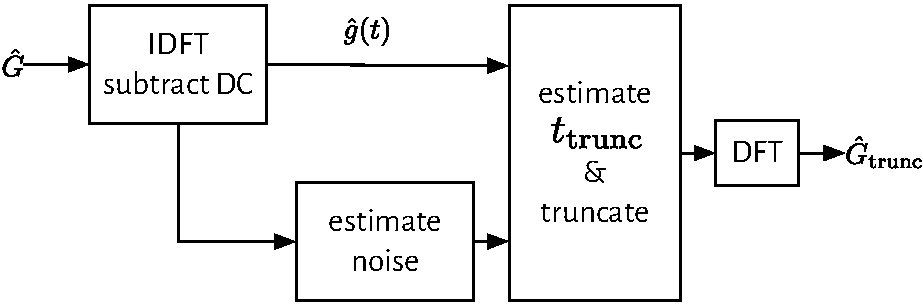
\includegraphics[width=\figurewidth]{\thisDir/figs/workflow-truncation.pdf}
   \caption{Workflow for impulse response truncation.}
   \label{fig:nparam:truncation:workflow}
 \end{figure} 

These procedures require that the following assumptions are satisfied.

\begin{assumption}
The estimate $\hat G_{\LPM}(\omega_k)$ is available at all frequencies $\omega_k$ for $k\in\{1,2,\dots,N/2\}$.
\end{assumption}

This assumption ensures that the impulse response corresponding to the \gls{FRF} can be computed (up to its mean value). It requires that the input signal excites the whole unit circle. This is satisfied, for instance, by using white noise as an excitation signal.


\begin{assumption}\label{ass:trunc:impulseReponse:decay}
The impulse response $g(t)$ decays exponentially over time, i.e. 
\[
  \exists A \in \PositiveRealNumbers, 
  \exists a > 0 ,
  \exists t_0 > 0,
  \forall t > t_0: 
     \abs{g(t)} \leq A \exp(- a t) \text{.}
\]
\end{assumption}

\begin{assumption}\label{ass:trunc:impulseResponse:lastSegmentNoise}
Within $90\%$ of the measurement window, the impulse response decays to a level that is indistinguishable from the noise.
\end{assumption}

Note that \assref{ass:trunc:impulseReponse:decay} and \assref{ass:trunc:impulseResponse:lastSegmentNoise} exclude the possibility of considering a system that is a pure integrator.

\subsection{Obtaining the Impulse Response Function}

The estimated impulse response function  $\hat g_{{\LPM}\without \DC}(t)$ is obtained explicitly via the \gls{IDFT} of the \gls{LPM}-estimate $\hat G_{\LPM}(\omega_k)$ of the \gls{FRF}, \latin{viz}:
\begin{align}\label{eq:impRespiDFT}
\hat g_{{\LPM}\without \DC}(t) 
&= 
\frac{1}{\sqrt{N}}
\sum_{k=1}^{N-1}
\hat G_{\LPM}(\omega_k)e^{\frac{j2\pi kt}{N}}
\end{align}
where the estimated \gls{FRF} in the frequency band between  the Nyquist and the sample frequencies is obtained as follows:
\begin{align}
\hat G_{\LPM}(\omega_{N-k}) = \overline{\hat G_{\LPM}(\omega_k)},\ \text{for}\ k=1,\dots,N/2
\end{align}
(with $\conj{\hat G_{\LPM}}$ the complex conjugate of $\hat G_{\LPM}$) to ensure $\hat g_{\LPM}(t)$ to be real.

Smoothing of the estimated \gls{FRF} requires the correct estimate of the impulse response. 
Unfortunately, the \gls{LPM} presented in \secref{sec:nparam:LRM} and in \citep{Schoukens2009LPM} does not estimate the \gls{DC} value of the \gls{FRF}, hence the subscript ``$\without\DC$'' in equation \eqref{eq:impRespiDFT}. 
Consequently, the mean value of the corresponding estimated impulse response given in equation \eqref{eq:impRespiDFT} is not correct. 
This limitation is lifted by developing a simple estimator of the mean value, presented below.

\subsection{Estimating the \glsentrytext{DC} Value of the \glsentrytext{FRF}}\label{sec:nparam:trunc:DCvalueEst}
The correct mean value of the impulse response accounts for (i.e. estimates) the \gls{DC} value of the \gls{FRF}. A time-domain method is proposed for estimating the mean value of the impulse response in equation \eqref{eq:impRespiDFT}. %The first is a frequency-domain technique and the second is a time-domain technique.

According to \assref{ass:trunc:impulseReponse:decay}, the true impulse response tends to zero asymptotically; and by \assref{ass:trunc:impulseResponse:lastSegmentNoise}, the last $10\%$ of the estimated impulse response is noise, plus a constant value due to an inaccuracy in the    average value of the impulse response. The correct estimate of the mean value is obtained by shifting the whole signal such that the last $10\%$ of the impulse response is centered around 0.
To this end, the following procedure is executed:

\begin{enumerate}
\item Compute the mean value $m_{g10}$ of the last 10\% of the impulse response $\hat g_{{\LPM}\without \DC}(t)$, estimated by the \gls{LPM}, as %$\hat g_{\LPM}(t)$ as
\begin{align}
   m_{g10} 
   = 
   \frac{1}{\lceil0.1N - 1\rceil}
   \sum_{t=\lfloor0.9N\rfloor}^{N-1}
      \hat g_{{\LPM}\without \DC}(t)
\end{align}

\item Next, subtract the computed mean value $m_{g10}$ from $\hat g_{{\LPM}\without \DC}(t)$ to obtain the improved impulse response $\hat g_{\LPM}(t)$, \latin{viz}:
\begin{align}
\hat g_{\LPM}(t) = \hat g_{{\LPM}\without \DC}(t) - m_{g10},\ \text{for}\ t=0,1,\dots,N-1
\end{align}
\end{enumerate}

\subsection{Determining the Truncation Time of the Impulse Response}
In this section, two methods will be discussed to determine the truncation time, i.e. the time beyond which the measured impulse response cannot be separated from the noise level.
Specifically, the first method uses an $F$-test to distinguish between signal and noise.
The second method fits an exponential through a well-chosen subset of the data to obtain $\truncTime$. 

\subsubsection{Truncation Via the $F$-Test}
\label{sec:nonparametric:truncation:ftest}
To distinguish the part of the measured impulse response where the actual impulse response dominates from the part where the noise dominates, the estimated impulse response $\hat{g}_{\LPM}$ is split into smaller segments. 
One can then gradually determine if in each of these segments, the observed impulse response is dominated by the noise.

% 1) cut into NS segments of minimally NM samples
% 2) assume last segment == noise
%    start from back
% 3) F-test on Var, Var==RMS if dc == 0 (i.e. noise)
%    H0: s²(1) =  s²(2)
%    H1: s²(1) >  s²(2)
%    alpha >> ==> beta <<
% 4) if H1 and RMS(signal)/RMS(noise) < f
%    robustness, SNR
%    select segment i
% 5) refine until wanted resolution is obtained

\begin{enumerate}
  \item The impulse response $\hat{g}_{\LPM}(t)$ is split into $N_S$ segments of approximate equal lengths
$L_S = \floor{\frac{N}{N_S}}$. 
If necessary, the length of the first segment is reduced to allow for the others to have equal lengths.
The $i^{\text{th}}$ segment is denoted $\segm{\hat{g}}{i}$, for $i \in \left\{1,\ldots,N_S\right\}$.
  By \assref{ass:trunc:impulseResponse:lastSegmentNoise}, the last segment, $\segm{\hat{g}}{N_S}$, is noise when $L_S \leqslant 0.1N$.
  
  \item Iteration is then carried out from the last segment ($i = N_S$) towards the beginning of the impulse response. To determine whether the preceding segment $\segm{\hat{g}}{i-1}$ is completely dominated by noise,  both an $F$-test and an absolute criterion on the RMS are used.

  The $F$-test is suited to compare the variances of different segments $\segm{\hat{g}}{i}$ and $\segm{\hat{g}}{i-1}$ \citep{Parsons1974}, while accounting for the degrees of freedom in each segment.
  For zero-mean noise, these variances are the \gls{RMS} value of each noise segment.
  This has the advantage that a segment in which the impulse response still has a significant amplitude is likely to have a large \gls{RMS} value, which is more likely to be detected.
  Let $s^2(i)$ denote the mean square value of segment $\segm{\hat{g}}{i}$, \latin{viz}:
  \begin{equation}
    s^2(i) 
    \isdef \frac{1}{L_S} \sum_{j=1}^{L_S} \left(\segm{\hat{g}}{i}(j)\right)^2
    = \left( \rms{\hat{g}^{[i]}} \right)^2
           \text{.}
  \end{equation}
  Starting with the last segment ($i = N_S$), the following null hypothesis and the alternative hypothesis are formulated:
  \begin{align}
     \nullHypothesis &: s^2(i-1) = s^2(i)\\
     \altHypothesis    &: s^2(i-1) > s^2(i)
     \text{.}
  \end{align}
  As segment $\segm{\hat{g}}{i}$ has been tested and been classified as noise (or assumed to be noise if $i=N_S$), the null hypothesis effectively states that the segment $\segm{\hat{g}}{i-1}$ is also noise.
  The alternative case occurs when $\segm{\hat{g}}{i-1}$ has a significant change, which indicates the presence of the signal.
  Using the $F$-test on the \gls{RMS} values of the two segments with a high confidence level of $\alpha=0.999$ and the aforementioned hypotheses, we can determine whether $\segm{\hat{g}}{i-1}$ is likely to be part of the actual impulse response.
  In particular, the null hypothesis is rejected when the empirical $F$ statistic is high, i.e.
  \begin{equation}
    F \isdef \frac{s^2(i-1)}{s^2(i)} \geq \ICDF{\FDistribution} \left( \alpha; n_{i-1}, n_{i} \right)
  \end{equation}
  where $ \ICDF{\FDistribution}$ is the inverse \gls{CDF} of the \mbox{$F$-distribution} with $n_{i-1}$ and $n_{i}$ degrees of freedom~\citep{EncyclopediaOfMathematics}.
  In this case $n_{i-1}$ and $n_{i}$ are the respective number of samples in the $(i-1)^{\text{th}}$ and $i^{\text{th}}$ segment of the impulse response.

  The high level of confidence ($\alpha=0.999$) ensures that the probability of a Type~II error is smaller than $1-\alpha$~\citep{Parsons1974}.
  In our case, such an error means that a part of the actual impulse response would be falsely classified as noise, which could significantly increase the bias as information of the system is discarded.
  A Type~I error is less detrimental since, in that case, noise is falsely classified as a signal component and kept in the impulse response, thereby causing a sub-optimal value of the variance of the estimate.
  As the \gls{LPM} samples are correlated over a short frequency span, the actual noise present in $\hat{g}$ may be slightly non-stationary.
  To cope with this, one can introduce other criteria which must be satisfied together with the outcome of the $F$-test.
  A criterion that shows good results is to check whether the segment $\segm{\hat{g}}{i-1}$ has an RMS value that is at least a factor $\kappa$ larger than the RMS of the noise.
  Even for a moderate $\kappa = 1.1$, a large improvement in the detection was observed. 
%  \JL{Q: doesn't this increase the probability of a Type II error?}
%  \EG{A: This slightly increases for small $\kappa$ and increases significantly for large values of $\kappa$. But it is needed to overcome nonstationarity of the noise.}

  \item This procedure is repeated until a segment $\segm{\hat{g}}{\starred{i}-1}$ is found that is dominated by the actual impulse response according to the outcome of the $F$-test and the absolute \gls{RMS} value of the segment.
  At that point, it is very likely that the transition from noise to the actual impulse response happens within the segment $\segm{\hat{g}}{\starred{i}-1}$.
  One now has the choice to accept the last sample of $\segm{\hat{g}}{\starred{i}-1}$ to be the last meaningful sample $\truncTime$ for the impulse response.
  The accuracy of this estimate is limited by the length of the segment $L_S$.

  \item
  A more accurate estimate can be obtained by dividing the segment $\segm{\hat{g}}{\starred{i}-1}$ -- which may contain both the signal and noise -- yet again into smaller segments.
  The procedure described above is then repeated until a satisfactory, accurate $\truncTime$ is obtained, or until the subsegments have a length that is too short ($L_{S\min} = 10$) to guarantee the accuracy of the RMS values. %rely on the RMS values to be accurate.
  To start this refinement, the last $\segm{\hat{g}}{\starred{i}}$ should be used to compare the RMS with the $F$-test, since the last subsegment of $\segm{\hat{g}}{\starred{i}-1}$ cannot be asserted to be dominated by noise.

\end{enumerate}
This procedure is illustrated in \figref{fig:nparam:trunc:nonparametric:truncation:Ftest} for the system described by the following equations:
\begin{subequations}
\label{eq:trunc:systemODEs}
\begin{align}
y_0(t)  &= 1.5371y_0(t-1)    -0.9025y_0(t-2) + u(t)\\
y(t)       &= y_0(t) + e(t),
\end{align}
\end{subequations}
where $e(t)$ is a white noise sequence, such that the \gls{SNR} of the output signal is $78.2\unit{dB}$.
The figure shows segments of the estimated impulse response. The last two segments are dominated by the noise, while all samples at $t<80$ have large system contributions. The algorithm outlined above selects $\truncTime = 80$, beyond which all samples are set to zero, resulting in a smoothed \gls{FRF} estimate. 

\begin{figure}[tbh]
\centering
 \setlength\figurewidth{0.68\columnwidth}
 \setlength\figureheight{0.68\figurewidth}
  % This file was created by matlab2tikz v0.2.2.
% Copyright (c) 2008--2012, Nico Schlömer <nico.schloemer@gmail.com>
% All rights reserved.
%
% The latest updates can be retrieved from
%   http://www.mathworks.com/matlabcentral/fileexchange/22022-matlab2tikz
% where you can also make suggestions and rate matlab2tikz.
%
%
%
\begin{tikzpicture}

\begin{axis}[%
width={\figurewidth},
height={\figureheight},
scale only axis,
xmin=0, xmax=160,
xtick={0,40,120,160},
extra x ticks={80},
extra x tick labels={$\truncTime$},
xlabel={Time $t$ \axisunit{samples}},
ymin=-1.3, ymax=1.7,
ylabel={Impulse Response $g$ \noaxisunit},
xmajorgrids,
legend style={nodes=right},
unbounded coords=jump]
\addplot [G0Hat]
coordinates{
 (0,1)(1,1.5371322893124)(2,1.46027567484678)(3,0.857375)(4,-9.19403442267708e-17)(5,-0.7737809375)(6,-1.18940366388567)(7,-1.12993348069139)(8,-0.663420431289062)(9,2.58473797920544e-16)(10,0.598736939238379)(11,0.920337882107388)(12,0.874320988002018)(13,0.513342083279504)(14,-2.97288235695525e-16)(15,-0.463291230159753)(16,-0.712139909233819)(17,-0.676532913772128)(18,-0.397214318458218)(19,3.70688722772794e-16)(20,0.358485922408542)(21,0.551040286598109)(22,0.523488272268203)(23,0.307356867725023)(24,-3.69062419514066e-16)(25,-0.277389573121834)(26,-0.426384469564153)(27,-0.405065246085946)(28,-0.237826885255332)(29,3.25911173049143e-16)(30,0.214638763942937)(31,0.329928174594791)(32,0.313431765865051)(33,0.184025910235575)(34,-3.30708767662391e-16)(35,-0.166083383987607)(36,-0.255292132245621)(37,-0.242527525633339)(38,-0.142395741346374)(39,2.46276523480082e-16)(40,0.128512156565103)(41,0.19754018542539)(42,0.187663176154121)(43,0.110183110235005)(44,-1.57683653460861e-16)(45,-0.0994402569870922)(46,-0.152852829872382)(47,-0.145210188378763)(48,-0.085257590334308)(49,1.08691267791672e-16)(50,0.0769449752767131)(51,0.11827460599818)(52,0.112360875698271)(53,0.0659706981778718)(54,-9.03953561309789e-18)(55,-0.0595385551055293)(56,-0.0915186355117147)(57,-0.086942703736129)(58,-0.0510468686836032)(59,-3.37119113007212e-17)(60,0.0460697989869518)(61,0.0708153755849754)(62,0.0672746068057266)(63,0.0394990939064379)(64,6.96464370550376e-17)(65,-0.0356479322505601)(66,-0.0547955877095567)(67,-0.052055808324079)(68,-0.030563645913324)(69,-6.6223576915183e-17)(70,0.0275836904367748)(71,0.0423997812287643)(72,0.0402797921673261)(73,0.0236495665882299)(74,7.47171997937755e-17)(75,-0.0213437338458773)(76,-0.032808142468988)(77,-0.0311677353455387)(78,-0.0182995838061092)(79,-1.10264207974723e-16)(80,0.0165153743850134)(81,0.0253863152372871)(82,0.0241169994754228)(83,0.014159869113351)(84,1.09491713926827e-16)(85,-0.0127792818747991)(86,-0.0196434468039785)(87,-0.0186612744637796)(88,-0.010956636797406)(89,-9.
04008618451361e-17)(90,0.00988836470965878)(91,0.0151997246837138)(92,0.0144397384495282)(93,0.00847803669294386)(94,1.089870940485e-16)(95,-0.00765142811538167)(96,-0.011761257215506)(97,-0.0111731943547307)(98,-0.00656014318042556)(99,-6.94431491476966e-17)(100,0.00592052922033389)(101,0.0091006366343929)(102,0.00864560480267328)(103,0.00507611374028394)(104,8.28330459778925e-17)(105,-0.00458119265060614)(106,-0.00704189914680743)(107,-0.00668980418946712)(108,-0.00392780004881355)(109,-4.17417836406919e-17)(110,0.00354483954405415)(111,0.00544888732359714)(112,0.0051764429574173)(113,0.00303925680408351)(114,2.99646375420681e-17)(115,-0.00274292926568532)(116,-0.00421624514158486)(117,-0.00400543288450561)(118,-0.00235171897916694)(119,-1.51313965697508e-17)(120,0.00212242637869816)(121,0.00326245011838534)(122,0.00309932761246606)(123,0.00181971531643633)(124,1.34170018845081e-17)(125,-0.00164229307308376)(126,-0.00252442171115117)(127,-0.00239820062559361)(128,-0.00140806102353516)(129,2.98195402915553e-17)(130,0.00127077507374057)(131,0.00195334939829986)(132,0.00185568192838489)(133,0.00108953077884828)(134,8.01099519434303e-17)(135,-0.000983301527910587)(136,-0.00151146452868156)(137,-0.00143589130224749)(138,-0.000843058147492346)(139,-1.34370239721807e-17)(140,0.000760859978111791)(141,0.00116954244000115)(142,0.00111106531800114)(143,0.000652342323733666)(144,5.27699411142e-17)(145,-0.000588738947169537)(146,-0.000904969645670134)(147,-0.00085972116338667)(148,-0.000504770054829573)(149,-5.87227774375603e-17)(150,0.000455554974483582)(151,0.000700248260835645)(152,0.000665235847793916)(153,0.000390581446247955)(154,6.47222614612674e-17)(155,-0.000352499755238696)(156,-0.000541838755752168)(157,-0.000514746817964564)(158,-0.000302224477647856)(159,-5.72914901895746e-17)(160,0.000272757591077104)(161,0.000419264500399693)
};
\addlegendentry{True Value};

\addplot [color=lightgray!80!black,solid]
coordinates{
 (0,1.0530788305713)(1,1.5401750859347)(2,1.45802774931507)(3,0.86442459854892)(4,-0.00639046554012114)(5,-0.770899909268136)(6,-1.18642954089334)(7,-1.0988342169306)(8,-0.68506381347042)(9,0.0399708891574246)(10,0.582041248283753)(11,0.959424942889007)(12,0.868352149881463)(13,0.534339065002973)(14,-0.0219200884705951)(15,-0.449211924918872)(16,-0.721946250583923)(17,-0.669426778593483)(18,-0.373376001506991)(19,-0.0022709676474749)(20,0.350322200100093)(21,0.571403202780426)(22,0.554205136082806)(23,0.29909565187015)(24,-0.0237986799431506)(25,-0.304203990253186)(26,-0.42813701795974)(27,-0.367058311722921)(28,-0.262557190612986)(29,-0.0274661695854109)(30,0.214175682648701)(31,0.310962412196269)(32,0.311037958803447)(33,0.209104758359952)(34,-0.00671904544159164)(35,-0.140494255746866)(36,-0.244750270738285)(37,-0.262875783709227)(38,-0.132322023640012)(39,0.00465465753686413)(40,0.115106772116674)(41,0.203431970436252)(42,0.182567654517998)(43,0.102159013124422)(44,-0.0107930930701593)(45,-0.0875488023510008)(46,-0.176735503357052)(47,-0.154047657658991)(48,-0.0947508213911722)(49,0.0205217625161969)(50,0.0997857617656283)(51,0.0911535793373973)(52,0.0962798164812225)(53,0.100578841992491)(54,0.0218501379371979)(55,-0.0411361498567127)(56,-0.0979354125787488)(57,-0.0941558858726104)(58,-0.0578038943961262)(59,-0.00247128921399623)(60,0.0371278788838963)(61,0.0426006567812478)(62,0.0583295959870679)(63,0.0287880172912928)(64,0.0301903935276118)(65,-0.0449464000912856)(66,-0.0431775699553004)(67,-0.0460879462916128)(68,-0.0109525225196768)(69,0.0259314140642792)(70,0.0393948296460815)(71,0.0734869744237198)(72,0.0126729865460558)(73,0.0210051418814731)(74,-0.00869414240387733)(75,-0.0037755930378919)(76,-0.0454813480527951)(77,-0.0345628267483219)(78,-0.0235173536721714)(79,-0.0191423884800511)(80,0.0139275469015572)(81,-0.0249685037417402)(82,0.0453234250443737)(83,-0.0363632237008142)(84,0.0526588455311864)(85,-0.00871880635556728)(86,0.00463223578390932)(87,-0.00295275845366561)(88,0.00226087007098701)(89,0.
0223031498517009)(90,0.00930507847920215)(91,0.0424493033614078)(92,0.0210554804986187)(93,0.0137926092452841)(94,-0.00879273684783215)(95,-0.0427631467397175)(96,0.0169742643303203)(97,-0.0102483098273445)(98,0.00702007059731766)(99,0.00389680308259893)(100,0.0200203386030399)(101,-0.0149723885519309)(102,0.0206932320549459)(103,-0.00990016880749287)(104,0.0122169096634572)(105,0.0326093021489499)(106,-0.0158280378400942)(107,-0.00384069310189821)(108,-0.0189978612360518)(109,0.00361300963961247)(110,-0.0086414779648314)(111,0.00967489049278187)(112,0.0127767263747594)(113,0.0223467406790162)(114,0.0220451436115617)(115,-0.0158533266301636)(116,-0.0327964043145136)(117,0.00160788974757907)(118,-0.015110510620568)(119,0.0213032326112286)(120,0.0023400304500529)(121,-0.00470808405409158)(122,-0.0116699533631736)(123,0.0439627790305935)(124,0.00405244981816977)(125,-0.00984448738347365)(126,0.0188834343586767)(127,0.016776623851269)(128,-0.0230014411021799)(129,-0.0257812870197883)(130,-0.0115513955393953)(131,0.0228515414156505)(132,-0.0018548544080748)(133,0.0170199205246556)(134,-0.00242844944846287)(135,-0.0103573115285161)(136,0.00143309952240079)(137,-0.0141897295156295)(138,0.0240191779599644)(139,0.00108024180330641)(140,0.0228388372432649)(141,0.0271013681331801)(142,0.00534558063780137)(143,-0.00249336000305963)(144,0.00561667226430895)(145,-0.00532193212122067)(146,0.00774716772437572)(147,-0.0153978136373772)(148,0.0101929461603683)(149,-0.0187856514764983)(150,0.0042812902722015)(151,0.0204403243691005)(152,0.00316252335774176)(153,0.027806894789268)(154,-0.0023256911611946)(155,0.0479062715493156)(156,0.0293056334746769)(157,-0.00149486623807802)(158,-0.000558253064721262)(159,0.0156180853939494)(160,0.0517576654594346)(161,-0.00540006188689709)
};
\addlegendentry{$\estimated g$};

\addplot [
color=black,
solid,
line width=1pt
]
coordinates{
 (0,1.0530788305713)(1,1.5401750859347)(2,1.45802774931507)(3,0.86442459854892)(4,-0.00639046554012114)(5,-0.770899909268136)(6,-1.18642954089334)(7,-1.0988342169306)(8,-0.68506381347042)(9,0.0399708891574246)(10,0.582041248283753)(11,0.959424942889007)(12,0.868352149881463)(13,0.534339065002973)(14,-0.0219200884705951)(15,-0.449211924918872)(16,-0.721946250583923)(17,-0.669426778593483)(18,-0.373376001506991)(19,-0.0022709676474749)(20,0.350322200100093)(21,0.571403202780426)(22,0.554205136082806)(23,0.29909565187015)(24,-0.0237986799431506)(25,-0.304203990253186)(26,-0.42813701795974)(27,-0.367058311722921)(28,-0.262557190612986)(29,-0.0274661695854109)(30,0.214175682648701)(31,0.310962412196269)(32,0.311037958803447)(33,0.209104758359952)(34,-0.00671904544159164)(35,-0.140494255746866)(36,-0.244750270738285)(37,-0.262875783709227)(38,-0.132322023640012)(39,0.00465465753686413)(40,0.115106772116674)(41,0.203431970436252)(42,0.182567654517998)(43,0.102159013124422)(44,-0.0107930930701593)(45,-0.0875488023510008)(46,-0.176735503357052)(47,-0.154047657658991)(48,-0.0947508213911722)(49,0.0205217625161969)(50,0.0997857617656283)(51,0.0911535793373973)(52,0.0962798164812225)(53,0.100578841992491)(54,0.0218501379371979)(55,-0.0411361498567127)(56,-0.0979354125787488)(57,-0.0941558858726104)(58,-0.0578038943961262)(59,-0.00247128921399623)(60,0.0371278788838963)(61,0.0426006567812478)(62,0.0583295959870679)(63,0.0287880172912928)(64,0.0301903935276118)(65,-0.0449464000912856)(66,-0.0431775699553004)(67,-0.0460879462916128)(68,-0.0109525225196768)(69,0.0259314140642792)(70,0.0393948296460815)(71,0.0734869744237198)(72,0.0126729865460558)(73,0.0210051418814731)(74,-0.00869414240387733)(75,-0.0037755930378919)(76,-0.0454813480527951)(77,-0.0345628267483219)(78,-0.0235173536721714)(79,-0.0191423884800511)(80,0)(81,0)(82,0)(83,0)(84,0)(85,0)(86,0)(87,0)(88,0)(89,0)(90,0)(91,0)(92,0)(93,0)(94,0)(95,0)(96,0)(97,0)(98,0)(99,0)(100,0)(101,0)(102,0)(103,0)(104,0)(105,0)(106,0)(107,0)(108,0)(109,0)(110,0)(111,0)(112,0)(113,0)(
114,0)(115,0)(116,0)(117,0)(118,0)(119,0)(120,0)(121,0)(122,0)(123,0)(124,0)(125,0)(126,0)(127,0)(128,0)(129,0)(130,0)(131,0)(132,0)(133,0)(134,0)(135,0)(136,0)(137,0)(138,0)(139,0)(140,0)(141,0)(142,0)(143,0)(144,0)(145,0)(146,0)(147,0)(148,0)(149,0)(150,0)(151,0)(152,0)(153,0)(154,0)(155,0)(156,0)(157,0)(158,0)(159,0)(160,0)(161,0)
};
\addlegendentry{$\estimated g_{\trunc}$};

\addplot [
color=gray,
densely dotted
]
coordinates{
 (0,0.628802731910641)(1,0.628802731910641)(2,0.628802731910641)(3,0.628802731910641)(4,0.628802731910641)(5,0.628802731910641)(6,0.628802731910641)(7,0.628802731910641)(8,0.628802731910641)(9,0.628802731910641)(10,0.628802731910641)(11,0.628802731910641)(12,0.628802731910641)(13,0.628802731910641)(14,0.628802731910641)(15,0.628802731910641)(16,0.628802731910641)(17,0.628802731910641)(18,0.628802731910641)(19,0.628802731910641)(20,0.628802731910641)(21,0.628802731910641)(22,0.628802731910641)(23,0.628802731910641)(24,0.628802731910641)(25,0.628802731910641)(26,0.628802731910641)(27,0.628802731910641)(28,0.628802731910641)(29,0.628802731910641)(30,0.628802731910641)(31,0.628802731910641)(32,0.628802731910641)(33,0.628802731910641)(34,0.628802731910641)(35,0.628802731910641)(36,0.628802731910641)(37,0.628802731910641)(38,0.628802731910641)(39,0.0795043572643008)(40,0.0795043572643008)(41,0.0795043572643008)(42,0.0795043572643008)(43,0.0795043572643008)(44,0.0795043572643008)(45,0.0795043572643008)(46,0.0795043572643008)(47,0.0795043572643008)(48,0.0795043572643008)(49,0.0795043572643008)(50,0.0795043572643008)(51,0.0795043572643008)(52,0.0795043572643008)(53,0.0795043572643008)(54,0.0795043572643008)(55,0.0795043572643008)(56,0.0795043572643008)(57,0.0795043572643008)(58,0.0795043572643008)(59,0.0795043572643008)(60,0.0795043572643008)(61,0.0795043572643008)(62,0.0795043572643008)(63,0.0795043572643008)(64,0.0795043572643008)(65,0.0795043572643008)(66,0.0795043572643008)(67,0.0795043572643008)(68,0.0795043572643008)(69,0.0795043572643008)(70,0.0795043572643008)(71,0.0795043572643008)(72,0.0795043572643008)(73,0.0795043572643008)(74,0.0795043572643008)(75,0.0795043572643008)(76,0.0795043572643008)(77,0.0795043572643008)(78,0.0795043572643008)(79,0.0795043572643008)(80,0.0214125686888731)(81,0.0214125686888731)(82,0.0214125686888731)(83,0.0214125686888731)(84,0.0214125686888731)(85,0.0214125686888731)(86,0.0214125686888731)(87,0.0214125686888731)(88,0.0214125686888731)(89,0.0214125686888731)(90,0.0214125686888731)(
91,0.0214125686888731)(92,0.0214125686888731)(93,0.0214125686888731)(94,0.0214125686888731)(95,0.0214125686888731)(96,0.0214125686888731)(97,0.0214125686888731)(98,0.0214125686888731)(99,0.0214125686888731)(100,0.0214125686888731)(101,0.0214125686888731)(102,0.0214125686888731)(103,0.0214125686888731)(104,0.0214125686888731)(105,0.0214125686888731)(106,0.0214125686888731)(107,0.0214125686888731)(108,0.0214125686888731)(109,0.0214125686888731)(110,0.0214125686888731)(111,0.0214125686888731)(112,0.0214125686888731)(113,0.0214125686888731)(114,0.0214125686888731)(115,0.0214125686888731)(116,0.0214125686888731)(117,0.0214125686888731)(118,0.0214125686888731)(119,0.0214125686888731)(120,0.0214125686888731)(121,0.0193285829589688)(122,0.0193285829589688)(123,0.0193285829589688)(124,0.0193285829589688)(125,0.0193285829589688)(126,0.0193285829589688)(127,0.0193285829589688)(128,0.0193285829589688)(129,0.0193285829589688)(130,0.0193285829589688)(131,0.0193285829589688)(132,0.0193285829589688)(133,0.0193285829589688)(134,0.0193285829589688)(135,0.0193285829589688)(136,0.0193285829589688)(137,0.0193285829589688)(138,0.0193285829589688)(139,0.0193285829589688)(140,0.0193285829589688)(141,0.0193285829589688)(142,0.0193285829589688)(143,0.0193285829589688)(144,0.0193285829589688)(145,0.0193285829589688)(146,0.0193285829589688)(147,0.0193285829589688)(148,0.0193285829589688)(149,0.0193285829589688)(150,0.0193285829589688)(151,0.0193285829589688)(152,0.0193285829589688)(153,0.0193285829589688)(154,0.0193285829589688)(155,0.0193285829589688)(156,0.0193285829589688)(157,0.0193285829589688)(158,0.0193285829589688)(159,0.0193285829589688)(160,0.0193285829589688)(161,0.0193285829589688)
};
\addlegendentry{$\mathrm{RMS} (\segm{\estimated g}{i})$};

% \addplot [color=black,dotted,forget plot]
% table[row sep=crcr]{
% 39	-1.5\\
% 39	 2.0\\
% nan nan\\
% 80	-1.5\\
% 80	 2.0\\
% nan nan\\
% 121 -1.5\\
% 121 2\\
% };

\addplot [truncationline] table[row sep=crcr]{
80	-1.5\\
80	 2.0\\
};

\node[annotation] at (axis cs: 20,-1.1) {Segment 1};
\node[annotation] at (axis cs: 60,-1.1) {Segment 2};
\node[annotation] at (axis cs: 100,-1.1) {Segment 3};
\node[annotation] at (axis cs: 140,-1.1) {Segment 4}; 

\end{axis}


\end{tikzpicture}%

\caption[Illustration of impulse response truncation using the $F$-test.]{Illustration of truncating the impulse response by performing an $F$-test on successive segments of the impulse response.}
\label{fig:nparam:trunc:nonparametric:truncation:Ftest}
\end{figure}

\subsubsection{Truncation Via Exponential Fitting}
\label{sec:nonparametric:truncation:exponentialfit}

The \gls{FRF} estimate is smoothed by truncating the estimated impulse response function. 
The truncation is applied at the time index beyond which the signal is indistinguishable from the noise.

This is done via the fit of an exponential function on the maxima of the impulse response, implemented as follows.

\begin{enumerate}
\item Obtain the estimate of the impulse response $\hat g_{\LPM}(t)$ from the \gls{LPM}, corrected for its \gls{DC} value as discussed in \secref{sec:nparam:trunc:DCvalueEst}. 
Henceforth, $\hat g_{\LPM}(t)$ will simply be denoted as $\hat g(t)$.

\item Obtain an estimate $\hat \sigma_\mathrm{n}$ of the standard deviation of the noise from the last 10\% of the data, \latin{viz}:
\begin{align}
\hat \sigma^2_\mathrm{n}=\frac{1}{\lceil0.1N - 1\rceil}\sum_{t=\lfloor0.9N\rfloor}^{N-1}\hat g^2(t).
\end{align}
This is valid, as per \assref{ass:trunc:impulseResponse:lastSegmentNoise}.

%This assumes that the impulse response of the system is not longer than 90\% of the length of the measured time interval.

\item Obtain $\mathbb{T}_\mathrm{HSNR}$ as the set of time instants where $\hat g(t)$ is significantly above the standard deviation of the noise. Only samples with absolute values of at least $5\hat\sigma_\mathrm{n}$ are retained: %Only samples with an absolute value of at least $5\hat\sigma_\mathrm{n}$ have been retained:
\begin{align}
\mathbb{T}_\mathrm{HSNR} = \left\{
t:|\hat g(t)|\geqslant 5\hat\sigma_\mathrm{n}
\right\}.
\end{align}
(Subscript HSNR stands for High \gls{SNR}.)

%This choice leaves a probability of $6\times10^{-7}$ of retaining a pure noise sample, in the case of Gaussian noise.

\item Find the set $\mathbb{T}_\mathrm{max}$ of indices corresponding to monotonically decreasing maxima of the impulse response:
\begin{align}\label{eq:TmaxDef}
\mathbb{T}_\mathrm{max} = \left\{
t: \left| \hat g(t)\right|>
\left|\hat g(t')\right|,
t < t' < N \land t'\in\mathbb{T}_\mathrm{HSNR}
\right\},
\end{align}

\item Fit an exponential function $Ae^{at}$ approximating $\hat g(t)$, in $t_\mathrm{max}\in\mathbb{T}_\mathrm{max}$. 
This is done by solving the following expression
\begin{align}\label{eq:expFit}
\ln \left|\hat g(t)\right|\approx \ln A+at,\ \mathrm{with}\ t\in\mathbb{T}_\mathrm{max},
\end{align}
for $\ln A$ and $a$ in a least squares sense.
This is a quadratic problem in the parameters and, thus, amount to a convex optimization problem that can be solved directly.
Since  $\ln \left|\hat g(t)\right|$ decreases for an increasing $t$ in $\mathbb{T}_\mathrm{max}$ (by construction in equation \eqref{eq:TmaxDef}), the estimated $a$ from equation \eqref{eq:expFit} is always negative.

\item
Determine the first time-instant $\truncTime$ at which the estimated exponential gets significantly below the noise floor, \latin{viz}:
\begin{align}\label{eq:truncTimeExpFit}
\truncTime = \min \left\{t:Ae^{at} < \gamma\hat\sigma_\mathrm{n}\right\}
\end{align}
where the parameter $\gamma$ can be tuned such that an appropriate trade-off between the decreased variance and the increased bias on the estimated smoothed FRF is found. This is discussed below. 

\item
 Truncate the estimated impulse response for $t \geqslant \truncTime$.

\end{enumerate}
  
\begin{figure}[tbh] %top bottom here
\centering
\setlength\figurewidth{0.85\columnwidth}
\setlength\figureheight{0.68\figurewidth}
% This file was created by matlab2tikz.
%
%The latest updates can be retrieved from
%  http://www.mathworks.com/matlabcentral/fileexchange/22022-matlab2tikz-matlab2tikz
%where you can also make suggestions and rate matlab2tikz.
%
\begin{tikzpicture}
% \pgfplotsset{compat=newest}
\pgfplotsset{tick style={black!30},grid style={black!10}}
\pgfplotsset{every axis legend/.append style={font=\footnotesize}}
\pgfplotsset{every axis label/.append style={font=\footnotesize}}
\pgfplotsset{every tick label/.append style={font=\footnotesize}}
\pgfplotsset{every axis title/.append style={font=\footnotesize}}
\pgfplotsset{every axis post/.style={unbounded coords=jump}}
\pgfplotsset{every axis title/.append style={at={(0.5,0.95)}}}

\definecolor{LPMTrunc}{named}{TangoSkyBlue2}
\definecolor{LPMTruncInit}{named}{TangoSkyBlue2}
\definecolor{RFIR}{named}{TangoScarletRed3}
\definecolor{RFIRInit}{named}{TangoScarletRed1}
\definecolor{existing}{named}{TangoChameleon3}
\definecolor{G0Hat}{named}{TangoOrange2}
\definecolor{GVXI}{named}{G0Hat}
\definecolor{reference}{named}{black}

\definecolor{heuristic}{named}{TangoPlum2}
\definecolor{observed}{named}{TangoOrange3}

\definecolor{best}{named}{TangoAluminium6}

\definecolor{G0HatFill}{named}{TangoOrange1}
\definecolor{GVXIFill}{named}{G0HatFill}
\definecolor{LPMTruncFill}{named}{TangoSkyBlue1}
\definecolor{RFIRFill}{named}{TangoScarletRed1}
\definecolor{existingFill}{named}{TangoChameleon1}
\definecolor{bestFill}{named}{TangoAluminium3}

\definecolor{FRFMean}{named}{TangoPlum3}
\definecolor{FRFSingle}{named}{TangoPlum1}
\definecolor{FRFNoise}{named}{TangoChocolate1}

\pgfplotsset{FRFMean/.style={color=FRFMean,mark=*,mark options={solid},only marks,medsmallmarkers}}
\pgfplotsset{FRFSingle/.style={color=FRFSingle,mark=square*,mark options={solid},only marks,smallmarkers}}
\pgfplotsset{FRFNoise/.style={color=FRFNoise,mark=x,mark options={solid},only marks,smallmarkers}}

\pgfset{number format/1000 sep={\,}}

\pgfplotsset{bandwidth/.style={area style,fill=TangoButter1,draw=TangoButter2,fill opacity=0.5}}
\pgfplotsset{goodestimate/.style={color=TangoChameleon2,line join=round}}
\pgfplotsset{badestimate/.style={color=TangoScarletRed2,solid,line join=round}}
\pgfplotsset{exact/.style={color=black,dashed,line width=0.75pt,line join=round}}

\pgfplotsset{LPMTruncmark/.append style={mark=*,mark options={solid}}}
\pgfplotsset{RFIRmark/.append style={mark=square*,mark options={solid}}}
\pgfplotsset{existingmark/.append style={mark=triangle*,mark options={solid}}}
\pgfplotsset{existingInitmark/.append style={mark=triangle,mark options={solid}}}
\pgfplotsset{LPMTruncInitmark/.append style={mark=o,mark options={solid}}}
\pgfplotsset{RFIRInitmark/.append style={mark=square,mark options={solid}}}
\pgfplotsset{bestmark/.append style={mark=diamond*,mark options={solid}}}
\pgfplotsset{G0Hatmark/.append style={mark=asterisk,mark options={solid}}}

\pgfplotsset{GVXI/.style={color=GVXI,line width=1pt}}
\pgfplotsset{G0Hat/.style={color=G0Hat,line width=1.5pt}}
\pgfplotsset{existing/.style={color=existing}}
\pgfplotsset{LPMTruncInit/.style={color=LPMTruncInit,densely dashed}}
\pgfplotsset{LPMTrunc/.style={color=LPMTrunc}}
\pgfplotsset{RFIRInit/.style={color=RFIRInit,densely dashed}}
\pgfplotsset{RFIR/.style={color=RFIR}}
\pgfplotsset{best/.style={color=best}}

\pgfplotsset{smallmarkers/.append style={mark size=0.75pt}}
\pgfplotsset{medsmallmarkers/.append style={mark size=0.5pt}}
\pgfplotsset{tinymarkers/.append style={mark size=0.25pt}}
\pgfplotsset{extremelytinymarkers/.append style={mark size=0.05pt}}


\tikzset{annotation/.style={align=left,draw=black!0.2,font=\scriptsize,fill=white,fill opacity=0.8}}
% http://tex.stackexchange.com/questions/83487/pgfplotstable-converting-zeros-to-in-a-knitr-inline-table
\pgfplotstableset{%
	zerofill=true,
	after row=[3pt],
                  every head row/.style={before row=\toprule, after row={\\\midrule}},
                  every last row/.style={after row=\bottomrule}
	assign column name/.code={%
        \pgfkeyssetvalue{/pgfplots/table/column name}{\multicolumn{1}{c}{\multirow{2}{*}{#1}} }%
    },
	columns/method/.style={string type,column name={\shortstack{\textsc{Method}\\\phantom{0}}}},
	columns/P000/.style={column type=r,column name={\shortstack[r]{\textsc{Min.}\\{$0\%$}}}},
	columns/P025/.style={column type=r,column name={\shortstack[r]{\vphantom{?}\\\textsc{$25\%$}}}},
	columns/P050/.style={column type=r,column name={\shortstack[r]{\textsc{Median}\\{$50\%$}}}},
	columns/P075/.style={column type=r,column name={\shortstack[r]{\vphantom{?}\\\textsc{$75\%$ }}}},
	columns/P100/.style={column type=r,column name={\shortstack[r]{\textsc{Max.}\\{$100\%$}}}},
	columns/contribution/.style={column name={\shortstack[r]{\textsc{Contribution}\\ \vphantom{0}}},
                    	postproc cell content/.append code={\pgfkeysalso{@cell content/.add={}{\%}}},
	}
}

\begin{axis}[%
width=\figurewidth,
height=\figureheight,
% scale only axis,
xmin=0,
xmax=1024,
xtick={ 0, 1024},
xlabel={Time $t$ \axisunit{samples}},
ymin=-5,
ymax=41,
ytick={-10,0,40},
extra y ticks={1.87,9.37},
extra y tick labels={{$\noiseStd$},{$5\noiseStd$}},
extra x ticks={704},
extra x tick labels={$\truncTime$},
ylabel={Impulse response $g(t)$ \noaxisunit},
ymajorgrids,
legend style={legend cell align=left},
]
\addplot [imprespFull] table{\thisDir/figs/expfit-full.tsv};
\addlegendentry{$g(t)$}

\addplot [imprespAbs] table{\thisDir/figs/expfit-abs.tsv};
\addlegendentry{$\abs{g(t)}$}

\addplot [imprespExpFit] table{\thisDir/figs/expfit-exp.tsv};
\addlegendentry{Exponential fit}

\addplot [imprespPeaks] table{\thisDir/figs/expfit-peaks.tsv};
\addlegendentry{Peaks}

\addplot [imprespTrunc] table{\thisDir/figs/expfit-result.tsv};
\addlegendentry{$g_{\trunc}(t)$}

\addplot [truncationline] table[row sep=crcr]{%
704	-28.3097809794082\\
704	40.7143028069402\\
};
\addlegendentry{$\truncTime$}

\addplot [imprespDetectLevel, forget plot] table[row sep=crcr]{%
0	9.37\\
1033.23	9.37\\
};
\addplot [imprespNoiseLevel, forget plot] table[row sep=crcr]{%
0	1.87\\
1033.23	1.87\\
};
\end{axis}
\end{tikzpicture}%

\caption[Impulse response truncation using exponential fit.]{Truncation of the impulse response $g(t)$ via the fit of  an exponential through the peaks of $\abs{g(t)}$ that are above $5\noiseStd$ with $\noiseStd$ is the estimated noise level, as per \eqref{eq:TmaxDef}.}
\label{fig:nparam:trunc:nonparametric:trunc:impresp:expfit}
\end{figure}

As an illustration, this procedure was applied to the noisy impulse response of the system described by the following difference equation:

\begin{equation}
y_0(t) = 2.583y_0(t - 1) -2.176y_0(t - 2)+0.592y_0(t-3) + u(t)
\end{equation}

The measured signal was disturbed by random white noise, $y(t) = y_0(t) + e(t)$, such that the \gls{SNR} was $14.2\unit{dB}$.
The result is depicted in \figref{fig:nparam:trunc:nonparametric:trunc:impresp:expfit}. 
An exponential function (black thick line) is fitted on the maxima (gray circles) of the absolute value of a noisy impulse response (dark gray line). The truncation time (black vertical line) $\truncTime$ was selected as the time instant at which the fitted exponential fell below $0.4\noiseStd$ (i.e. $\gamma = 0.4$ in equation \eqref{eq:truncTimeExpFit}).

\paragraph*{Considerations on the choice of $\gamma$}

\begin{itemize}
\item The tuning parameter $\gamma$ is application- and system-dependent.  A higher value lowers the variance of the estimated \gls{FRF}, but increases its bias, and vice versa.

\item The bias error is highest in the vicinity of (sharp) resonance peaks. 
If the latter is to be estimated with a high accuracy, a value $\gamma \ll 1$ must be used.

\item If one is interested in obtaining a smooth initial estimate of the \gls{FRF}, a (small) bias error is acceptable, and choosing $\gamma \approx 1$ was found to be a good rule of thumb.
\end{itemize}

\subsection{Simulation Results}
\label{sec:nparam:trunc:simResults}

\figref{fig:nparam:trunc:LPMvsTRunc} and \figref{fig:nparam:trunc:pdfAndRMSeVStruncTime} compare the \gls{LPM} with and without truncation of the impulse response.
Here, the truncation instant $\truncTime$ is determined using the exponential fitting method.
They were obtained from simulations on the system in \eqref{eq:trunc:systemODEs} where the noise variance was set such that the \gls{SNR} of the output signal is $18.3\unit{dB}$.

\begin{figure}
    \centering
    \setlength\figurewidth{0.85\columnwidth}
    \setlength\figureheight{0.68\figurewidth}
    \input{\thisDir/figs/figLPMvsTRunc.tikz}
    \caption[Comparison of FRF estimated using LPM and Truncated LPM.]{The bias $\sampleBias{\placeholder}$ and standard deviation $\sampleStd{\placeholder}$ of the \gls{FRF} estimates using both the \gls{LPM} (blue) and truncated~\gls{LPM} (red) are shown. 
    It can be seen that the truncation reduces the variance at the cost of an increased bias, however, the overall \gls{RMS} error is reduced by the truncation.}
    \label{fig:nparam:trunc:LPMvsTRunc}
\end{figure}


In \figref{fig:nparam:trunc:LPMvsTRunc} one observes the following:
\begin{itemize}
\item a decrease of the variance on the truncated estimate of about $10 \unit{dB}$ compared to the non-truncated \gls{LPM}, is observed.
Note also that the improvement in variance is proportional to the measurement time, i.e.
\begin{equation}
  \frac{\sampleStd{\trunc}}{\sampleStd{\LPM}} \approx \sqrt{\frac{\truncTime}{\Tm}}
\end{equation}
where $\Tm$ is the total measurement time.
Equivalently, this means that for \glspl{FRF} estimated with a finer frequency resolution, are improved more by truncation than coarsely spaced \glspl{FRF}.

\item an increase of the bias of the truncated estimate, especially in the vicinity of the resonance frequency. Still, this bias lies below the variance of the non-truncated estimate. As such, for a single experiment, the increase in bias still yields a better estimate when truncation is invoked.

This bias depends on the time instant at which the truncation is performed, as discussed below.

\item the error on the truncated \gls{LPM} estimate is strongly correlated over the frequency. This must be taken into account when formulating a maximum likelihood parametric estimator of the system.
It is, however, advised to use the raw data instead of such smoothed \glspl{FRF} to estimate a parametric model such that no bias is introduced into the parametric estimate.
In \chapref{sec:initvals}, however, it will be shown that smoothed \glspl{FRF} can lead to improved starting values.

\end{itemize}

\begin{figure}
   \centering
        \setlength\figurewidth{0.68\columnwidth}
        \setlength\figureheight{0.68\figurewidth}
        % This file was created by matlab2tikz.
%
\begin{tikzpicture}

\begin{axis}[%
width=0.951\figurewidth,
height=\figureheight,
at={(0\figurewidth,0\figureheight)},
scale only axis,
xmode=log,
xmin=10,
xmax=2048,
xtick={10,100,1000},
xticklabels={\empty},
xminorticks=true,
ymin=0,
ymax=500,
ytick={  0, 100, 200, 300, 400, 500},
ylabel={Number of realizations},
axis x line*=bottom,
axis y line*=right
]
\addplot[histogramSmootherFTest] plot table[] {\thisDir/figs/pdfs-3.tsv};
% \addplot[forget plot,color=white!15!black,solid,line width=2.0pt] table[] {\thisDir/figs/pdfs-4.tsv};

\addplot[histogramSmootherExpFit] plot table[] {\thisDir/figs/pdfs-5.tsv};
% \addplot[forget plot,color=white!15!black,solid,line width=2.0pt] table[] {\thisDir/figs/pdfs-6.tsv};

\end{axis}


\begin{axis}[%
width=0.951\figurewidth,
height=\figureheight,
at={(0\figurewidth,0\figureheight)},
scale only axis,
xmode=log,
xmin=10,
xmax=2048,
xminorticks=true,
xlabel={Truncation Time $\truncTime$ \axisunit{samples}},
ymin=0,
ymax=2.5,
ytick={  0, 0.5,   1, 1.5,   2, 2.5},
ylabel={RMS Error \noaxisunit},
legend style={legend cell align=left,align=left,draw=black}
]
\addplot [mainCurve] table[]{\thisDir/figs/pdfs-1.tsv};
\addlegendentry{RMS Error};

\addplot [pointOfInterest] table[]{\thisDir/figs/pdfs-2.tsv};
\addlegendentry{Theoretical optimum};

% \addlegendimage{empty legend}
% \addlegendentry{\textbf{Histograms using:}};

\addlegendimage{histogramSmootherFTest}
\addlegendentry{$F$-test};

\addlegendimage{histogramSmootherExpFit}
\addlegendentry{Exponential fitting};



\end{axis}
\end{tikzpicture}%

         \caption[RMS error of the FRF versus truncation time.]{
         The left y-axis shows the \gls{RMS} error of the estimated \gls{FRF} as a function of the chosen truncation time $\truncTime$.
         The corresponding optimal $\truncTime$ is indicated as well.
         Both bar plots (right y-axis) indicate for $\nMC =1000$ realizations of the disturbing noise and excitation signal, the number of times that $\truncTime$ has been selected by means of either the method using the $F$-test or the method that fits an exponential.
         It can be seen that both methods allow to almost halve the \gls{RMS} error and approach the optimal truncation time.}
   \label{fig:nparam:trunc:pdfAndRMSeVStruncTime}
\end{figure}

In \figref{fig:nparam:trunc:pdfAndRMSeVStruncTime}, the \gls{RMS} error of the estimated \gls{FRF} (without the \gls{DC} value) as a function of the time $\truncTime$ at which the impulse response is truncated, is shown.
To the left of the optimal truncation length, the \gls{RMS} error increases steeply.
In that region, one is essentially using a overly simplified impulse response to represent the system and hence the \gls{RMS} error is dominated by the bias error.
To the right hand side of the minimum, the \gls{RMS} error increases more gradually, due to an increase of the noise variance.

A good practice would be to truncate the impulse response at the minimizer (black dot) of the \gls{RMS} error. 
However, this minimizer is unknown in practice, since it depends on the true underlying system.
Nevertheless, the proposed approaches provide a reasonable way to approximate the optimal truncation length.

The truncation time is determined from the data as described in \secref{sec:nonparametric:truncation:exponentialfit}. 
This was done on $1000$ realizations of the noise, and depicted in \figref{fig:nparam:trunc:pdfAndRMSeVStruncTime} by the histogram.
Clearly, both methods for selecting the truncation time $\truncTime$ have a good overall performance, based on the mode of their distribution (around the $90^{\text{th}}$ sample). 

For the $F$-test based method, the obtained $\truncTime$ values only take a discrete set of values due to the limitation of the segment length.
While most trials result in $\truncTime \in \Set{70, 80, 90}$, a few outliers with much higher truncation times can be observed.
These outliers can be attributed to the high power of the $F$-tests.

For the exponential fitting approach, however, a closely grouped set of (continuous) values for $\truncTime$ is obtained around the $90^{\text{th}}$ sample, without significant outliers.
Although this distribution has a mode that is quite a bit higher than the method using the $F$-test, due to the absence of outliers, this method is more reliable to use for the particular system that we studied.

From the plot, we can conclude that the \gls{RMSE} increases rapidly when $\truncTime$ is smaller than the optimal.
On the other hand, selection of a value of $\truncTime$ that is too large, is not nearly as detrimental to the modeling error.
The graph also shows that the \gls{RMSE} of the model can be decreased from $0.62$ (without truncation) to $0.18$ when the optimal truncation is applied. 
Also, one observes a low sensitivity of the \gls{RMSE} w.r.t.~$\truncTime$, when truncating at times beyond that optimum. 
Therefore, a somewhat conservative truncation method is still likely to yield a close to optimal result.

\paragraph{Interaction of the truncation method and the system properties}
As seen in the previous simulation example, the exponential fitting method is well-suited to determine $\truncTime$ when the underlying system exhibits an exponential decay.
However, if the system under test is not part of this class of systems, the exponential fitting method may provide sub-optimal results or even be ineffective.

Consider instead that we are measuring a boxcar averager, i.e. a moving-average filter.
Such a system is governed by the difference equation:
\begin{align}
  y(t) = \sum_{i=0}^{\Nbc-1} \Nbc^{-1} u(t-i) 
  \text{,}
\end{align}
where $\Nbc = 88$.
Since this system is a trivial \gls{FIR}, it is easy to see that $\truncTime = \Nbc$ provides the optimal truncation point. 

We simulate the boxcar averager for a white noise input $u(t)$ and add white noise with standard deviation $\sigma_e \approx 0.1$ to the output $y(t)$ for $2\,048$ samples from which the first $1\,024$ samples are discarded to randomize the state of the system under test.
A single realization of the impulse response function is shown in \figref{fig:nparam:trunc:boxcar:impresp} together with the $\truncTime$ and other relevant quantities of the exponential fitting method.
It is easy to observe that the exponential fitting provides sub-optimal results since it truncates well past the end of the finite impulse response.

\begin{figure}
   \centering
        \setlength\figurewidth{0.68\columnwidth}
        \setlength\figureheight{0.68\figurewidth}
        % This file was created by matlab2tikz.
%
\begin{tikzpicture}

\begin{axis}[%
width=\figurewidth,
height=\figureheight,
at={(0\figurewidth,0\figureheight)},
scale only axis,
xmin=0,
xmax=1024,
xtick={0,1024},
extra x ticks={89,338},
extra x tick labels={{$\Nbc$},{$\truncTime$}},
extra y ticks={0.35},
extra y tick labels={$5\noiseStd$},
xlabel={Time \axisunit{samples}},
ymin=-0.17410927258308,
ymax=1.13796758214927,
ytick={-100,  -90,  -80,  -70,  -60,  -50,  -40,  -30,  -20,  -10,    0,   10,   20,   30,   40,   50,   60,   70,   80,   90,  100},
ylabel={Impulse response $g(t)$ \noaxisunit},
grid=major,
legend style={legend cell align=left},
]
\addplot [imprespFull]
  table[]{\thisDir/data/expfit-boxcar/full.tsv};

\addlegendentry{$g(t)$};

\addplot [imprespAbs]
  table[]{\thisDir/data/expfit-boxcar/abs.tsv};

\addlegendentry{$\abs{g(t)}$};

\addplot [imprespExpFit]
  table[]{\thisDir/data/expfit-boxcar/expfit.tsv};

\addlegendentry{Exponential fit};

\addplot [imprespPeaks]
  table[]{\thisDir/data/expfit-boxcar/peaks.tsv};
\addlegendentry{Peaks};

\addplot [truncationline, forget plot]
  table[]{\thisDir/data/expfit-boxcar/truncationTime.tsv};
\addplot [imprespNoiseLevel,forget plot]
  table[]{\thisDir/data/expfit-boxcar/noiseLevel.tsv};
\addplot [imprespDetectLevel,forget plot]
  table[]{\thisDir/data/expfit-boxcar/detectionLevel.tsv};
\end{axis}
\end{tikzpicture}%

         \caption[Exponential fit of boxcar averager]{Exponential fit of the impulse response of a boxcar averager. $\truncTime \gg \Nbc$ shows that a sub-optimal truncation point is found.}
         \label{fig:nparam:trunc:boxcar:impresp}
\end{figure}

By repeating the experiment above $\nMC = 1\,000$ times as a Monte Carlo simulation where both the input signal and disturbing noise are varied, we gain insight into the behavior of both truncation methods.
The histograms of the observed values of $\truncTime$ for both methods is shown in \figref{fig:nparam:trunc:boxcar:trunctime} together with the \gls{RMS} error as a function of $\truncTime$.
It can be seen that the $F$-test based method mostly selects the optimal truncation point.
On the other hand, the exponential fitting method is largely ineffective and doesn't truncate the response in most of the cases.

\begin{figure}
   \centering
        \setlength\figurewidth{0.68\columnwidth}
        \setlength\figureheight{0.68\figurewidth}
        % This file was created by matlab2tikz.
%
%The latest updates can be retrieved from
%  http://www.mathworks.com/matlabcentral/fileexchange/22022-matlab2tikz-matlab2tikz
%where you can also make suggestions and rate matlab2tikz.
%
\begin{tikzpicture}

\begin{axis}[%
width=\figurewidth,
height=\figureheight,
at={(0\figurewidth,0\figureheight)},
scale only axis,
xmode=log,
xmin=1,
xmax=1100,
xtick={10,100,1000},
xticklabels={\empty},
xminorticks=true,
ymin=0,
ymax=1000,
ylabel={Number of realizations},
axis x line*=bottom,
axis y line*=right,
legend style={nodes=right},
]
\addplot[histogramSmootherFTest] plot table[] {\thisDir/data/rmse-boxcar/histogram-F-test.tsv};

\addplot[histogramSmootherExpFit] plot table[] {\thisDir/data/rmse-boxcar/histogram-expFit.tsv};

\end{axis}

\begin{axis}[%
width=\figurewidth,
height=\figureheight,
at={(0\figurewidth,0\figureheight)},
scale only axis,
separate axis lines,
xmode=log,
xmin=1,
xmax=1100,
xminorticks=true,
xlabel={Truncation Time $\truncTime$ \axisunit{samples}},
ymin=0,
ymax=0.15,
y tick label style={
        /pgf/number format/.cd,
            fixed,
            precision=3,
        /tikz/.cd
    },
ytick={0,0.0577,0.101,0.135,0.150},
ylabel={RMS Error \noaxisunit},
legend style={legend cell align=left,align=left,draw=black},
legend pos=south west
]
\addplot [mainCurve] table[]{\thisDir/data/rmse-boxcar/rmse.tsv};
\addlegendentry{RMS Error};

\addplot [pointOfInterest] table[]{\thisDir/data/rmse-boxcar/optimum.tsv};
\addlegendentry{Optimum};

\addlegendimage{histogramSmootherFTest}
\addlegendentry{$F$-test};

\addlegendimage{histogramSmootherExpFit}
\addlegendentry{Exponential fitting};


\end{axis}
\end{tikzpicture}%

         \caption[RMS error of the FRF versus truncation time (boxcar)]{RMSE of a boxcar averager as a function of the truncation time $\truncTime$.
         Empirical histograms of $\truncTime$ as determined using both the $F$-test and exponential fitting are shown.
         For this system, the $F$-test based method is clearly superior.
         The exponential fitting method is not effective in most cases.}
         \label{fig:nparam:trunc:boxcar:trunctime}
\end{figure}

It can be seen that both the $F$-test method and the exponential fitting method each have their own strengths and weaknesses.
Particularly, the $F$-test method can only select $\truncTime$ from a discrete set of values, but works well for specifically designed \gls{FIR} filters where there is a clear jump in the amplitude of the impulse response.
On the other hand, the exponential fitting method relies on the exponential decay of the impulse response to obtain sensible values of $\truncTime$ and is hence a better match for `physical' systems.
One should remember, however, that for the studied examples, both approaches only very seldomly select a $\truncTime$ that increases the \gls{RMS} error on the impulse response compared to not truncating the response.
As such, a use has little to lose by trying out both methods: the model quality is very unlikely to decrease and the additional computational effort is minimal.

\begin{guideline}[Check and reinforce assumptions in the data.]
As illustrated by the presented smoothing operation, it pays off to check typical assumptions of the system (e.g. smoothness of the \gls{FRF}, finite support of the impulse response) and even reinforce such assumptions to improve the model quality.
For the truncation approaches, even if the assumptions do not hold, the methods are constructed such that the unavoidable model error is unlikely to increase.
\end{guideline}

\subsection{Conclusion}
\label{sec:nparam:trunc:conclusion}
This section introduced a time domain method to smooth the \gls{LPM}-estimate of an \gls{FRF}. 
It consisted of, after obtaining the \gls{FRF} from the \gls{LPM}, computing the associated estimated impulse response via the \gls{IDFT}.
Then, it was determined statistically at which time index the impulse response had decayed below the noise floor, yielding a point beyond which the response may be set to zero.

The different methods to determine $\truncTime$ presented in this section, essentially enforce different prior knowledge of the impulse response of the system.
The exponential fitting technique relies on the exponential decay present in most physical systems.
The $F$-test based technique is better suited for systems where a sudden jump in the impulse response is present.

The results clearly indicate that the truncation technique lowers the impact of the noise on the estimate of the \gls{FRF}, resulting in a decreased variance. 
A bias-variance trade-off is possible by tuning the time beyond which the impulse response is indistinguishable from the noise.



\section{Conclusions}
\label{sec:conclusion}
In this chapter, the performance of non-parametric \gls{LPM} and \gls{LRM} estimators were compared to observe the \gls{FRF} of resonant systems.
Since the \gls{LRM} is a biased estimator while the \gls{LPM} is asymptotically unbiased, it is important to compare their behavior.
Hence, expressions for the bias of the \gls{LRM} were derived.
For good \glspl{SNR} in resonant systems, it was seen that the \gls{LRM} is always superior to the \gls{LPM}.
For extremely poor \gls{SNR}, i.e. $\SNR \approx 10\unit{dB}$, the \gls{LPM} may perform slightly better than the \gls{LRM} when short measurement records are available.
In this chapter, the \gls{LRIC} was introduced.
This is an extension of the \gls{LRM} which solves the non-linear optimization problem and should thus be able to avoid a bias altogether.
However, it is seen that this estimator is extremely noisy but seems to provide a smaller bias than the \gls{LRM}.
Since the overall \gls{RMS} error for the \gls{LRIC} is much larger than most other methods, the \gls{LRIC} cannot be used in its current form.

Relatedly, two approaches to aid in performing the bias-variance trade-off for these local methods are illustrated.
First, a short study of cross-validation for local models is given.
Secondly, an approach to truncate the impulse response obtained from the \gls{LPM} is illustrated.
The latter can improve the performance of the \gls{LPM} considerably if a large number of noisy samples is measured.


% \begin{subappendices}
  \section{Proof of the \glsentrytext{LOOCV} statistic for linear models}

  We follow an approach similar to \citet{Hyndman2014LOOCV} and \citet[Section 12.3.2]{Seber2003} to prove that for a linear model, one can easily compute the \gls{PRESS}/\gls{LOOCV} statistic by means of the so-called `hat-diagonals', the diagonal entries of the hat matrix $H$.
  This is relevant, e.g. for local linear models used in the \gls{LRM} and hence also the \gls{LPM}.

  We consider the linear model
  \begin{equation}
    Z = K \theta + V
  \end{equation}
  with $Z \in \ComplexMatrix{N\times1}$, $\theta \in \ComplexMatrix{\nth \times 1}$, $K \in \ComplexMatrix{N \times \nth}$.
$V \in \ComplexMatrix{N \times 1}$ is a \gls{iid} complex gaussian random variable.
The least-squares solution of such a linear model is:
\begin{equation}
  \hat{\theta} = \left(K^{\HT} K \right)^{-1} K^{\HT} Z = \pinv{K} Z
\end{equation}
such that the estimated output $\hat{Z}$ is given by
\begin{equation}
  \hat{Z} = K \pinv{K} Z = H Z
\end{equation}
where $H$ is the so-called `hat matrix' that projects the measurements $Z$ onto the estimates $\hat{Z}$.

The \gls{PRESS} statistic used in \gls{LOOCV} is defined as~\citep[Chapter 12]{Seber2003}
\begin{equation}
  \PRESS \isdef 
    \frac{1}{N} 
      \sum_{i=1}^{N}
      \abs{
        Z_i - \ignoring{i}{\hat{Z}}
      }^2
\end{equation}
where $\hat{Z}_i$ is the $i^{\text{th}}$ row of $\hat{Z}$ and $\ignoring{i}{\hat{Z}}$ denotes the estimated $\hat{Z}_i$ when the $i^{\text{th}}$ data point (i.e. row) is removed from the estimation problem.
For linear models, this is equivalent to
\begin{equation}
  \PRESS_{\mathrm{linear}} = 
     \frac{1}{N}
     \sum_{i=1}^{N}
     \abs{
       \frac{Z_i - \hat{Z}_i}
                {1 - H_{ii}}
     }^2
     \text{.}
\end{equation}
Note that in this last expression, no terms $\ignoring{i}{\hat{Z}}$ occur, such that the statistic can be computed without having to compute $N$ additional linear models.
In this appendix, we prove that these last two expressions are equivalent for linear models.

\paragraph{Proof}
\TODO{proof}
Denote the design matrix $\ignoring{i}{K}$ to be the design matrix $K$ where the $i^{\text{th}}$ row has been removed:
\begin{equation}
  \ignoring{i}{K}
  \isdef
  \begin{bmatrix}
    K_{1,1} & K_{1,2} & \cdots & K_{1,\nth}\\
   && \vdots\\
    K_{i-1,1} & K_{i-1,1} & \cdots & K_{i-1,\nth}\\
    K_{i+1,1} & K_{i+1,1} & \cdots & K_{i+1,\nth}\\
    && \vdots\\
    K_{N,1} & K_{N,2} & \cdots & K_{N,\nth}\\
  \end{bmatrix}
\end{equation}

\begin{lemma}[Matrix Inversion Lemma]\label{lem:matrix-inversion-lemma}
The Woodbury formula, states that
\begin{equation*}
\left(A+UCV \right)^{-1} 
= 
A^{-1} - A^{-1} U \left(C^{-1}+VA^{-1}U \right)^{-1} VA^{-1}
\end{equation*}
when the dimensions of the matrices allow for the multiplications~\citep[Section 3.2.2]{matrixcookbook}.
\end{lemma}

\TODO{evt. Seber2003/ChristensenXXXX: QR decomposition to compute $H$}


\end{subappendices}

